\documentclass{name}
\usepackage{lipsum}
\usepackage{multicol}
\usepackage{listings}
\usepackage{longtable}
\usepackage{amsmath}
\usepackage{mathtools}
\usepackage{float}
\usepackage{amssymb}
\usepackage[utf8]{inputenc}
\usepackage{booktabs}
\usepackage{array}
\usepackage{caption}
\usepackage{subcaption}
\usepackage[a4paper,left=2cm,right=2cm,top=2cm,bottom=2cm]{geometry}
\usepackage{setspace}
\usepackage{stmaryrd}
\usepackage[sorting=none]{biblatex}
\addbibresource{bibliographie.bib}
\usepackage{csquotes}
\usepackage[english]{babel}
\NoAutoSpaceBeforeFDP
\usepackage[pdftex]{graphicx}
\usepackage{fancyhdr}
\usepackage{lmodern}
\usepackage{color}
\usepackage{xcolor}
\usepackage{algorithm}
\usepackage{algorithmic}
\usepackage{awesomebox}
\usepackage{todonotes}
\usepackage{upquote}
\usepackage{hyperref}
\newtheorem{theorem}{Théorème}
\newtheorem{remark}{Remarque}
\newtheorem{definition}{Définition}

% Configuration listings pour Python
\definecolor{codebg}{rgb}{0.95,0.95,0.97}
\definecolor{codegreen}{rgb}{0.0,0.5,0.0}
\definecolor{codegray}{rgb}{0.5,0.5,0.5}
\definecolor{codepurple}{rgb}{0.58,0,0.82}
\lstset{
  language=Python,
  basicstyle=\ttfamily\footnotesize,
  backgroundcolor=\color{codebg},
  keywordstyle=\color{blue}\bfseries,
  stringstyle=\color{codegreen},
  commentstyle=\color{codegray}\itshape,
  numberstyle=\tiny\color{codegray},
  numbers=left,
  numbersep=5pt,
  breaklines=true,
  frame=single,
  rulecolor=\color{gray!30},
  tabsize=4,
  showstringspaces=false,
  captionpos=b,
  aboveskip=8pt,
  belowskip=8pt,
}

\begin{document}
%----------- Informations du rapport ---------

\titre{Rapport Fil Rouge} %Titre du fichier .pdf

\eleves{Marin \textsc{Decanini}\\Nolan \textsc{Carlisi}\\ Mai 2025} %Noms des élèves

\enseignantenseirb{ \textsc{aa}\\\textsc{aa }}
\enseignant{Jordan  \textsc{Ramassamy-Moutoussamy}\\ENSEEIHT\\  } %Nom de l'enseignant



%----------- Initialisation -------------------
        
\fairemarges %Afficher les marges
\fairepagedegarde %Créer la page de garde

\newpage
\setcounter{pagezero}{\value{0}}

\begin{center}
	\begin{minipage}{13cm}
	    \begin{center}
	        \section*{Abstract}\\
	    \end{center}
		Ce rapport présente nos résultats et analyses concernant le projet Fil Rouge de l'UE Machine Learning. Le projet consiste en la conception d'un système de reconnaissance de commandes audio pour drones quadricoptères, à partir d'un corpus de 54 enregistrements de 18 locuteurs (13 hommes, 5 femmes) pour trois commandes : \textit{avance}, \textit{recule} et \textit{tournegauche}.
		
		Nous explorons successivement plusieurs familles de méthodes de classification — régression logistique multiclasse, machines à vecteurs de support (SVM), méthodes d'ensemble (Bagging, AdaBoost, Gradient Boosting, Random Forest) et réseaux de neurones (FNN et CNN avec PyTorch) — combinées à différentes méthodes de prétraitement spectral (FFT+PCA, STFT, MFCC).
		
		Notre étude personnelle (Partie V) constitue un benchmark exhaustif de \textbf{35\,668 expériences} croisant 9 méthodes de prétraitement, 10 classifiers et 3 méthodes d'évaluation. Les résultats montrent que la combinaison \textbf{MFCC Summary × Régression Logistique} atteint les meilleures performances avec une accuracy moyenne de 96.2\% en validation croisée.
	\end{minipage}
\end{center}



\par 
\setcounter{page}{\value{pagezero}}

\newpage
\setcounter{page}{\value{pagezero}}
\tableofcontents

%% ================================================================
%% SECTION 1 : PRÉAMBULE
%% ================================================================
\newpage
\section{Préambule : Choix architecturaux}

Ce préambule explique pourquoi nous avons décidé de développer une librairie supplémentaire autour du Notebook ainsi que les détails de comment cette librairie fonctionne et est architecturée.

\subsection{Librairie Python d'entraînement}

\subsubsection{Justification}

Jupyter Notebook se prêtant mal à du développement efficace (pas de refactoring, duplication de code, cellules exécutées dans le désordre...), nous avons pris le choix de développer autour du notebook une petite librairie Python modulaire. Par exemple, pour les questions demandant d'afficher des spectrogrammes STFT et MFCC, nous définissons une seule fonction \texttt{show\_subplots\_for\_transformed\_data} réutilisable :

\begin{lstlisting}[caption={Exemple d'appel API pour les spectrogrammes MFCC}]
X_mfcc = mfcc_coefficients(X, sr=fs, n_mfcc=13)
show_subplots_for_transformed_data(X_mfcc, y=y, genres=genres, method="mfcc", fs=fs)
plt.show()
\end{lstlisting}

Plus généralement, cela permet de transformer le notebook en simple consommateur de la librairie pour gagner en maintenabilité, reproductibilité et efficacité.

\subsubsection{Architecture et benchmarks}

Nous avons développé une architecture modulaire articulée autour de trois modules :

\begin{itemize}
    \item \textbf{\texttt{utils/preprocessings.py}} : 10 transformeurs compatibles scikit-learn (\texttt{FFTPCAFeatureExtractor}, \texttt{MFCCSummaryTransformer}, \texttt{WaveletTransformer}, etc.) avec une factory \texttt{make\_preprocessor(name)} et des grilles d'hyperparamètres par défaut.
    \item \textbf{\texttt{classifiers/}} : Registre de classifiers (LR, SVM, MLP, ensembles) avec \texttt{make\_classifier(name)} et \texttt{get\_classifier\_param\_grid(name)}.
    \item \textbf{\texttt{evaluation/}} : Orchestration des benchmarks via trois méthodes d'évaluation :
    \begin{itemize}
        \item \texttt{manual\_loo} : Leave-One-Out pédagogique avec preprocessing par fold
        \item \texttt{grid\_search\_cv} : \texttt{GridSearchCV} sklearn avec pipeline
        \item \texttt{train\_test} : Split train/test simple (80/20)
    \end{itemize}
\end{itemize}

On évalue un modèle de manière agnostique à son fonctionnement interne via :

\begin{lstlisting}[caption={API de benchmark unifié}]
result = run_grid_search(
    X_train=X, y_train=y,
    preprocessor="fft_pca",
    classifier="svm",
    preprocessor_param_grid={...},
    classifier_param_grid={...},
    cv=LeaveOneOut(),
)
\end{lstlisting}

Les méthodes d'ensemble sont traitées comme un cas particulier des classifiers prenant un \texttt{base\_classifier} en entrée, permettant de tester des combinaisons comme ``Bagging + SVM'' ou ``Bagging + NN''.

%% ================================================================
%% SECTION 2 : PREPROCESSING
%% ================================================================
\newpage
\section{Preprocessing}

Le corpus est constitué de 54 enregistrements audio (.wav) de commandes pour un drone, répartis en 3 classes (\textit{avance}, \textit{recule}, \textit{tournegauche}) par 18 locuteurs (M01--M13, F01--F05). Le plus court enregistrement contient 18\,522 échantillons à $f_s = 22\,050$ Hz. Tous les signaux sont recadrés à cette longueur par \texttt{energy\_trim} (centrage autour du barycentre d'énergie).

\begin{lstlisting}[caption={Chargement du dataset}]
X, y, genres, fs = load_dataset()
# X.shape = (54, 18522), y.shape = (54,), fs = 22050 Hz
\end{lstlisting}

\subsection{Représentation spectrale : Transformée de Fourier (FFT)}

\textbf{Question :} Appliquer une FFT sur $X$ et expliquer pourquoi la dimension résultante est trop grande pour une régression logistique.

La dimension après FFT est très élevée (18\,522 points, ou 9\,261 si on ne conserve que la moitié positive du spectre), alors que nous n'avons que 54 exemples. Il est impossible d'appliquer directement une régression logistique car :

\begin{enumerate}
    \item \textbf{Fléau de la dimensionnalité} : $P \gg N$ (18\,522 variables pour 54 observations).
    \item \textbf{Surapprentissage} : Le modèle a suffisamment de degrés de liberté pour mémoriser parfaitement le bruit du jeu d'entraînement.
    \item \textbf{Instabilité des coefficients} : La matrice de covariance $\hat{X}^T\hat{X}$ devient singulière, rendant l'estimation des $\beta$ instable voire impossible.
\end{enumerate}

C'est pourquoi une réduction de dimension (ACP) est indispensable.

\subsection{ACP sur $|\hat{X}|$}

On applique une ACP sur les magnitudes FFT $|\hat{X}|$ avec 20 composantes principales.

\begin{lstlisting}[caption={ACP sur les magnitudes FFT}]
X_fft = preprocess_fft(X)
pca = PCA(n_components=20, random_state=RANDOM_SEED).fit(X_fft)
plot_pca_explained_variance(pca)
\end{lstlisting}

\begin{figure}[H]
    \centering
    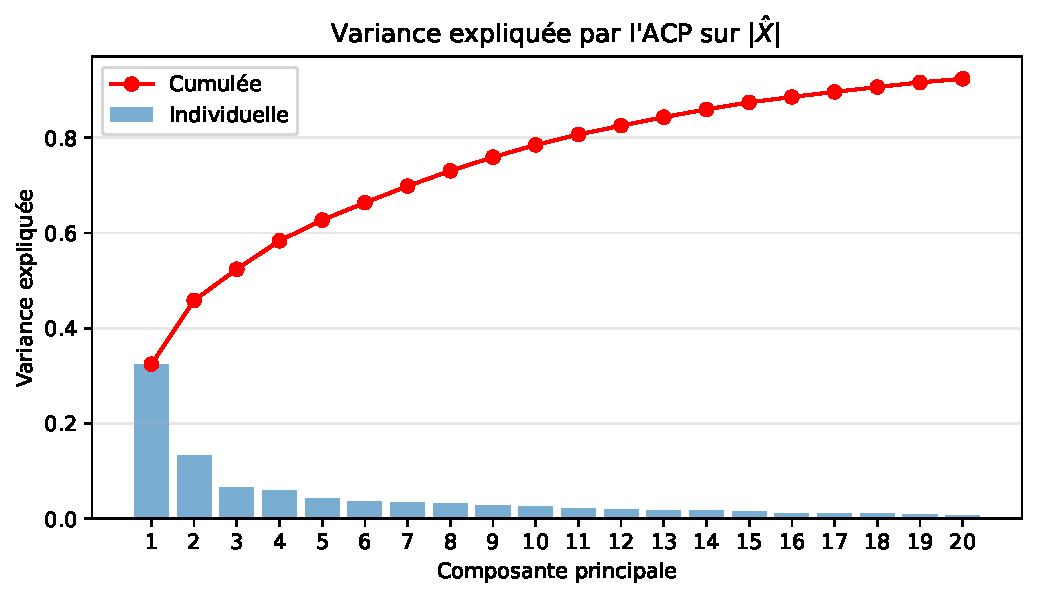
\includegraphics[width=0.85\textwidth]{figures/pca_explained_variance.pdf}
    \caption{Variance expliquée individuelle et cumulée par les 20 premières composantes principales de l'ACP appliquée sur $|\hat{X}|$. Les 5 premières composantes capturent la majorité de la variance.}
    \label{fig:pca_variance}
\end{figure}

\subsection{Short-Term Fourier Transform (STFT)}

La STFT calcule la transformée de Fourier sur des fenêtres glissantes, produisant une représentation temps-fréquence de dimension $(N, F, T)$ où $F$ est le nombre de fréquences et $T$ le nombre de pas temporels.

\begin{lstlisting}[caption={STFT et visualisation}]
X_stft = stft_magnitude(X, fs=fs, nperseg=400)
# X_stft.shape = (54, n_freqs, n_times)
show_subplots_for_transformed_data(X_stft, y=y, genres=genres, method="stft", fs=fs)
\end{lstlisting}

\begin{figure}[H]
    \centering
    \begin{subfigure}[b]{0.48\textwidth}
        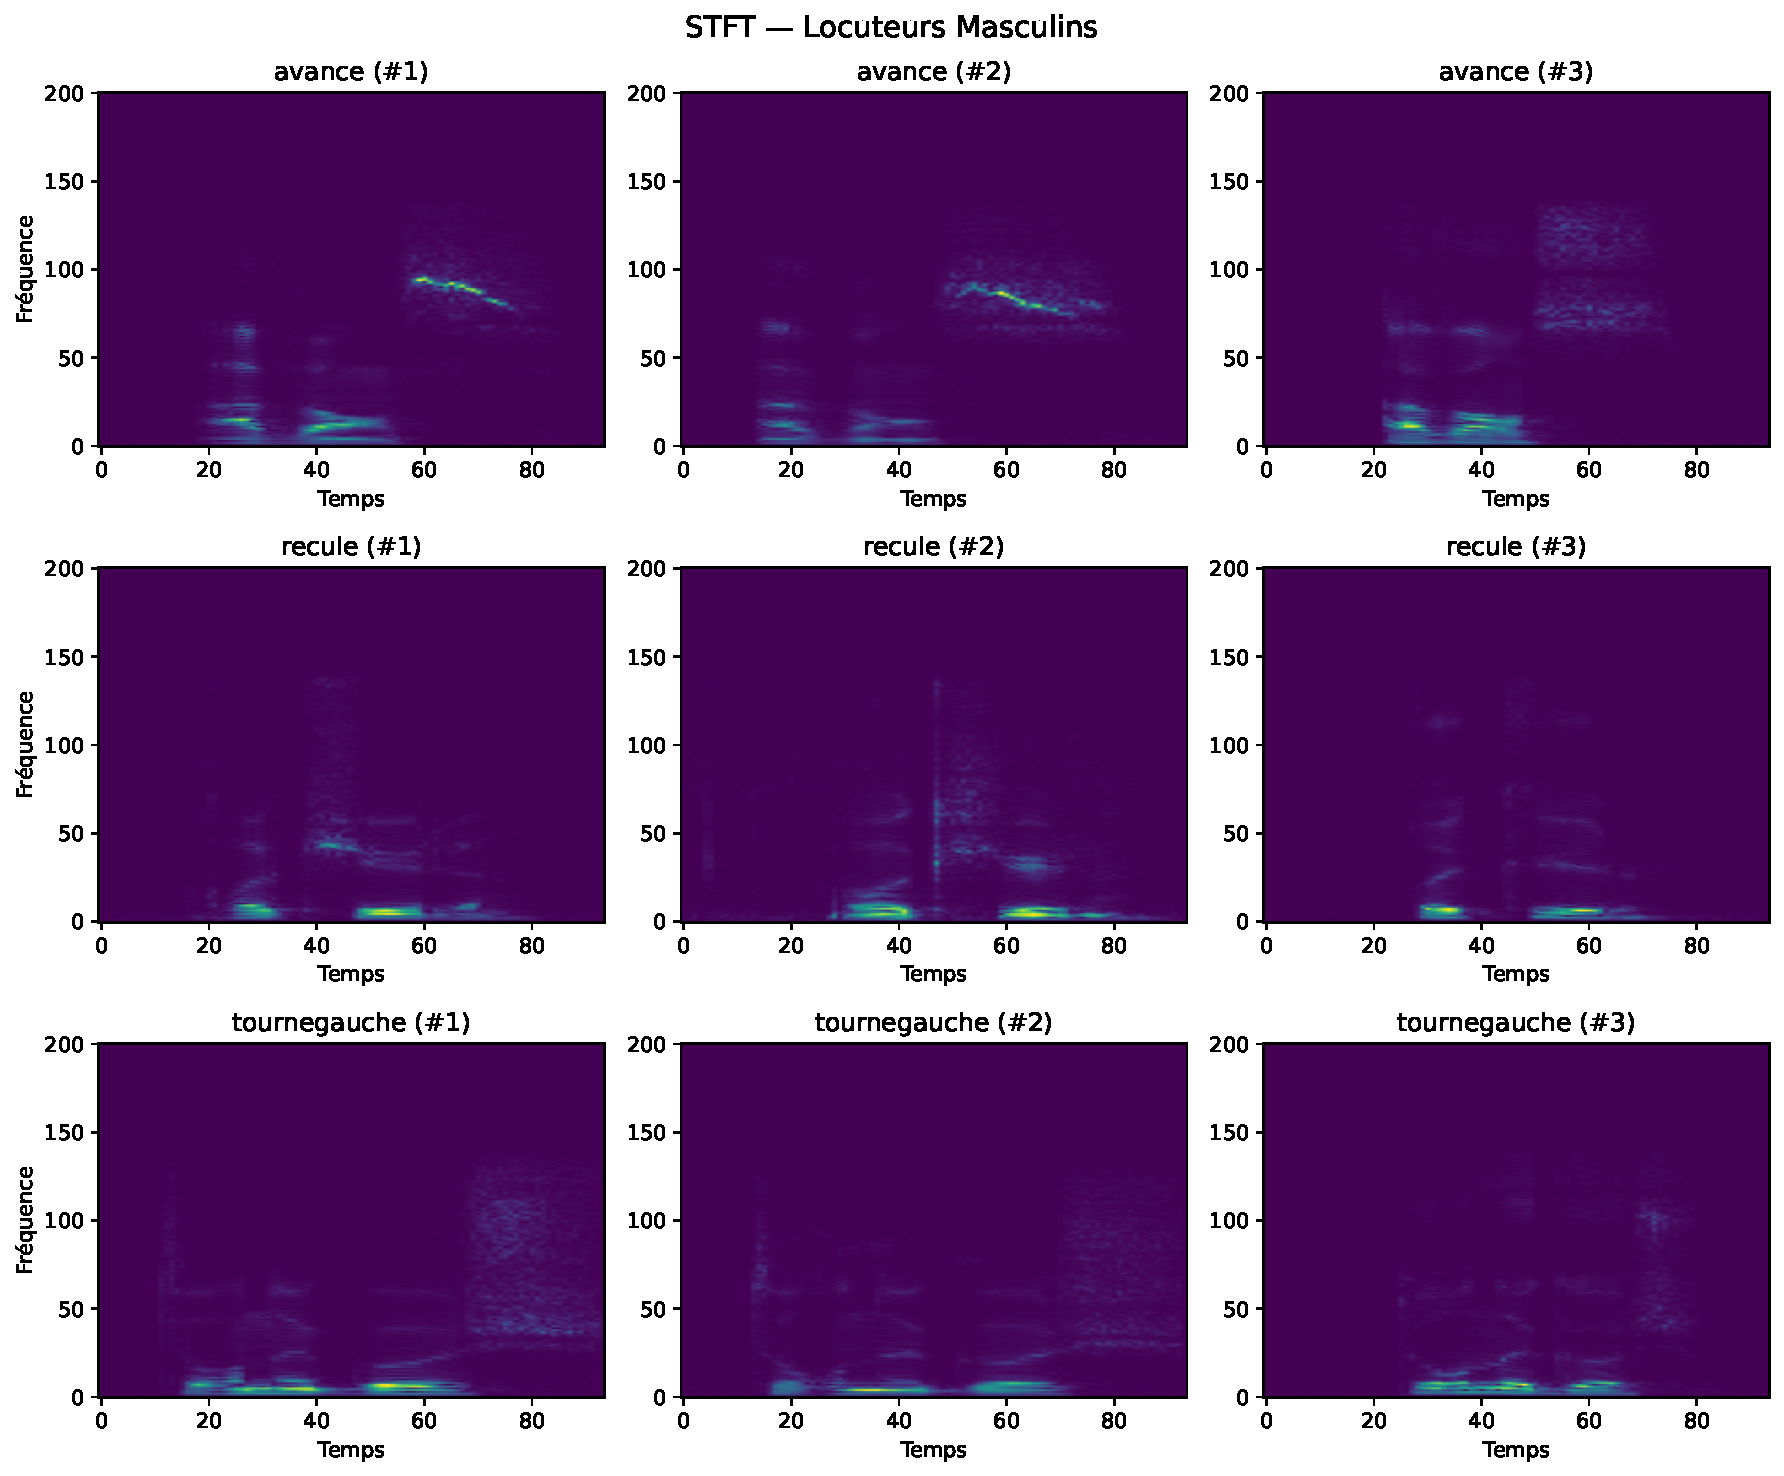
\includegraphics[width=\textwidth]{figures/stft_spectrograms_male.pdf}
        \caption{Locuteurs masculins}
    \end{subfigure}
    \hfill
    \begin{subfigure}[b]{0.48\textwidth}
        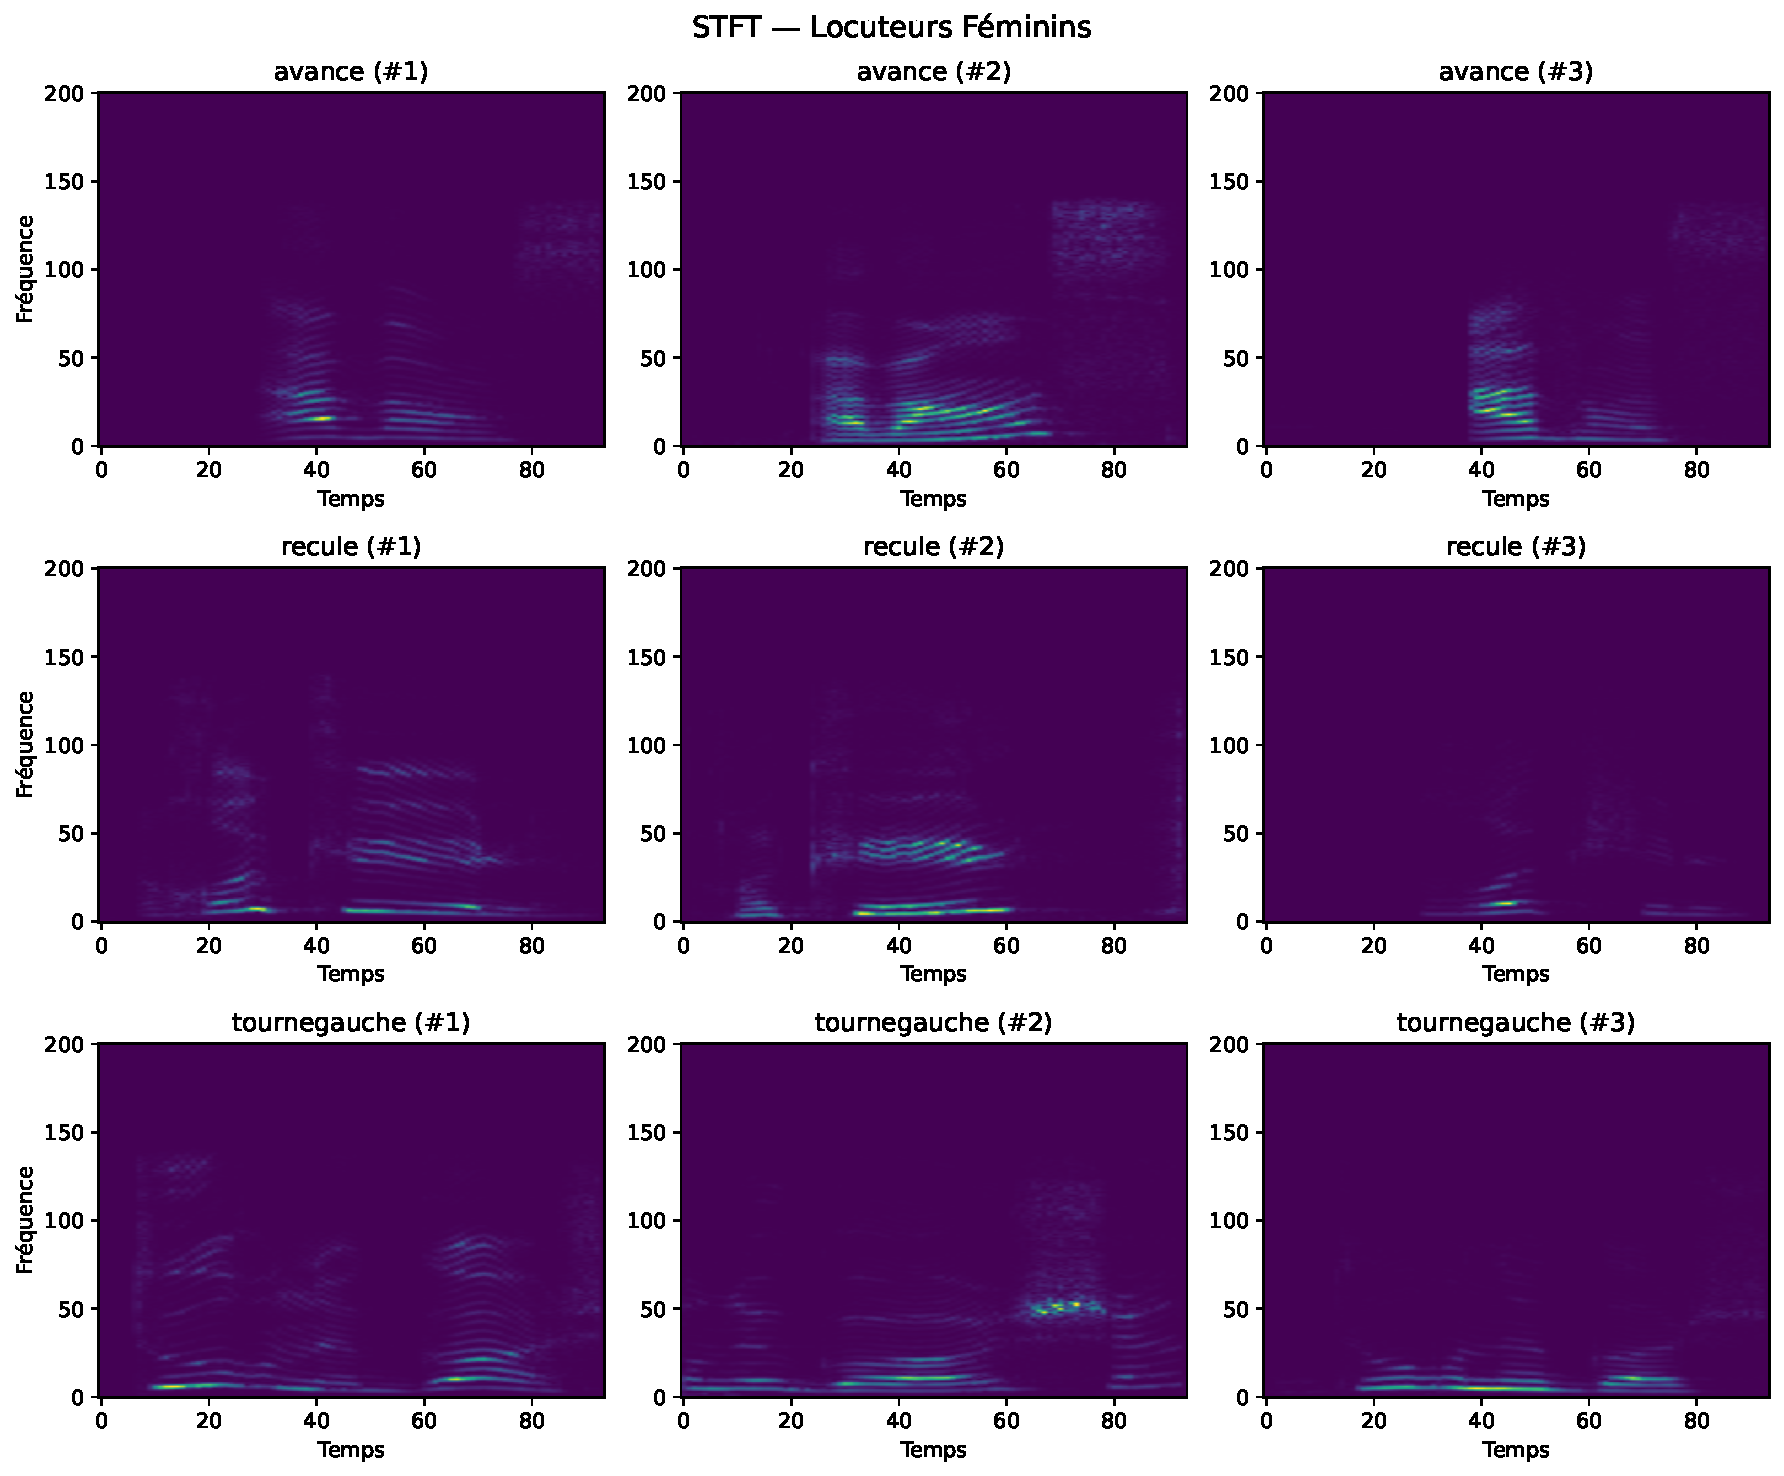
\includegraphics[width=\textwidth]{figures/stft_spectrograms_female.pdf}
        \caption{Locuteurs féminins}
    \end{subfigure}
    \caption{Spectrogrammes STFT de trois instances de chaque mot pour les locuteurs masculins et féminins. On observe des différences dans la distribution fréquentielle entre les mots et entre les genres.}
    \label{fig:stft_spectrograms}
\end{figure}

\subsection{MFCC (Mel-Frequency Cepstral Coefficients)}

Les MFCC modélisent la perception humaine de la hauteur sonore via l'échelle de Mel. On calcule 13 coefficients cepstraux par fenêtre temporelle.

\begin{lstlisting}[caption={MFCC et visualisation}]
X_mfcc = mfcc_coefficients(X, sr=fs, n_mfcc=13)
# X_mfcc.shape = (54, 13, n_times)
show_subplots_for_transformed_data(X_mfcc, y=y, genres=genres, method="mfcc", fs=fs)
\end{lstlisting}

\begin{figure}[H]
    \centering
    \begin{subfigure}[b]{0.48\textwidth}
        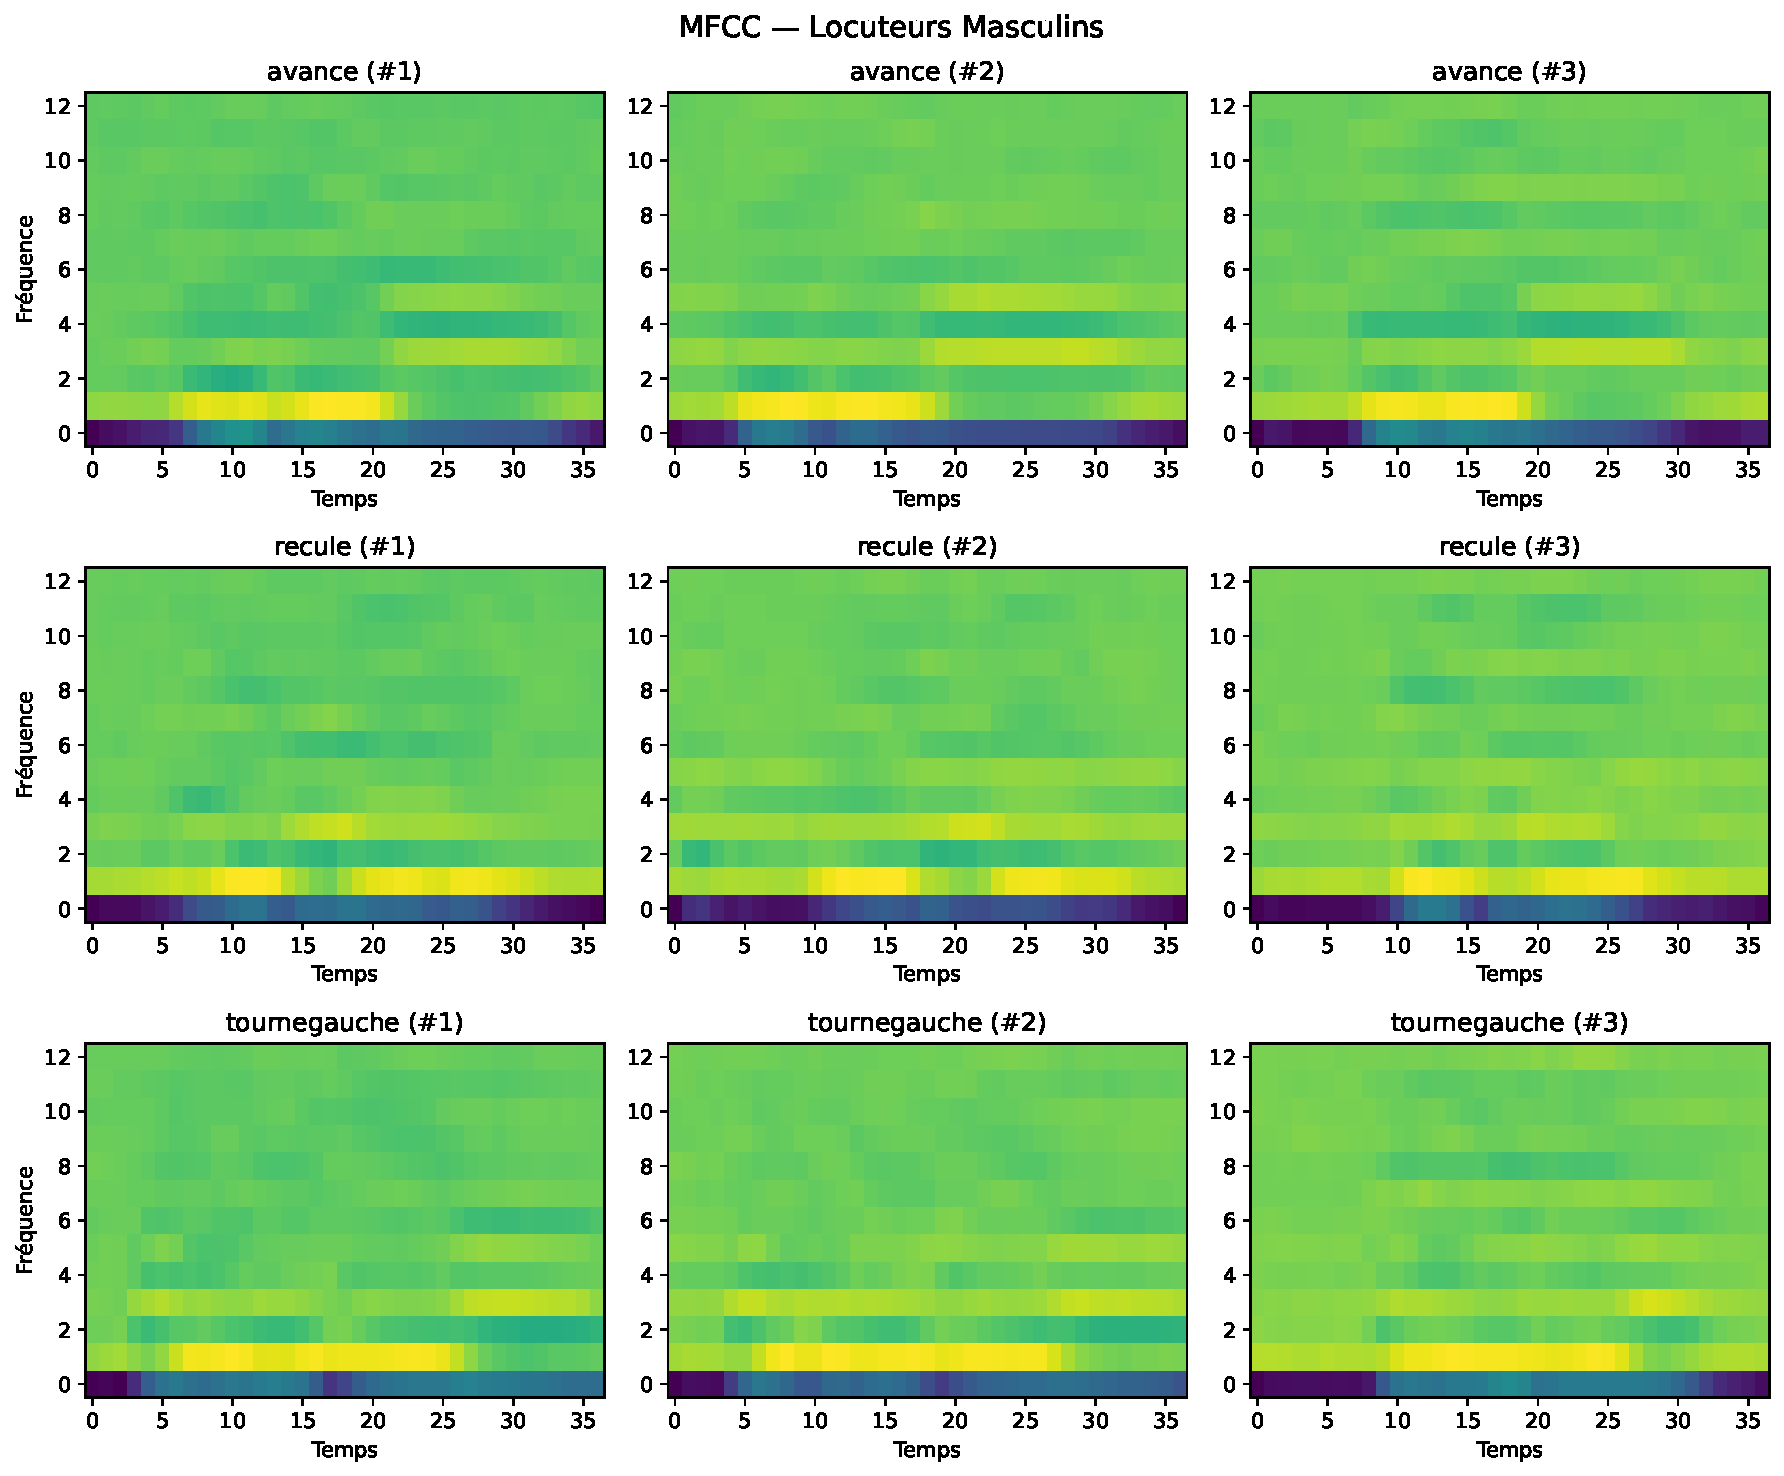
\includegraphics[width=\textwidth]{figures/mfcc_spectrograms_male.pdf}
        \caption{Locuteurs masculins}
    \end{subfigure}
    \hfill
    \begin{subfigure}[b]{0.48\textwidth}
        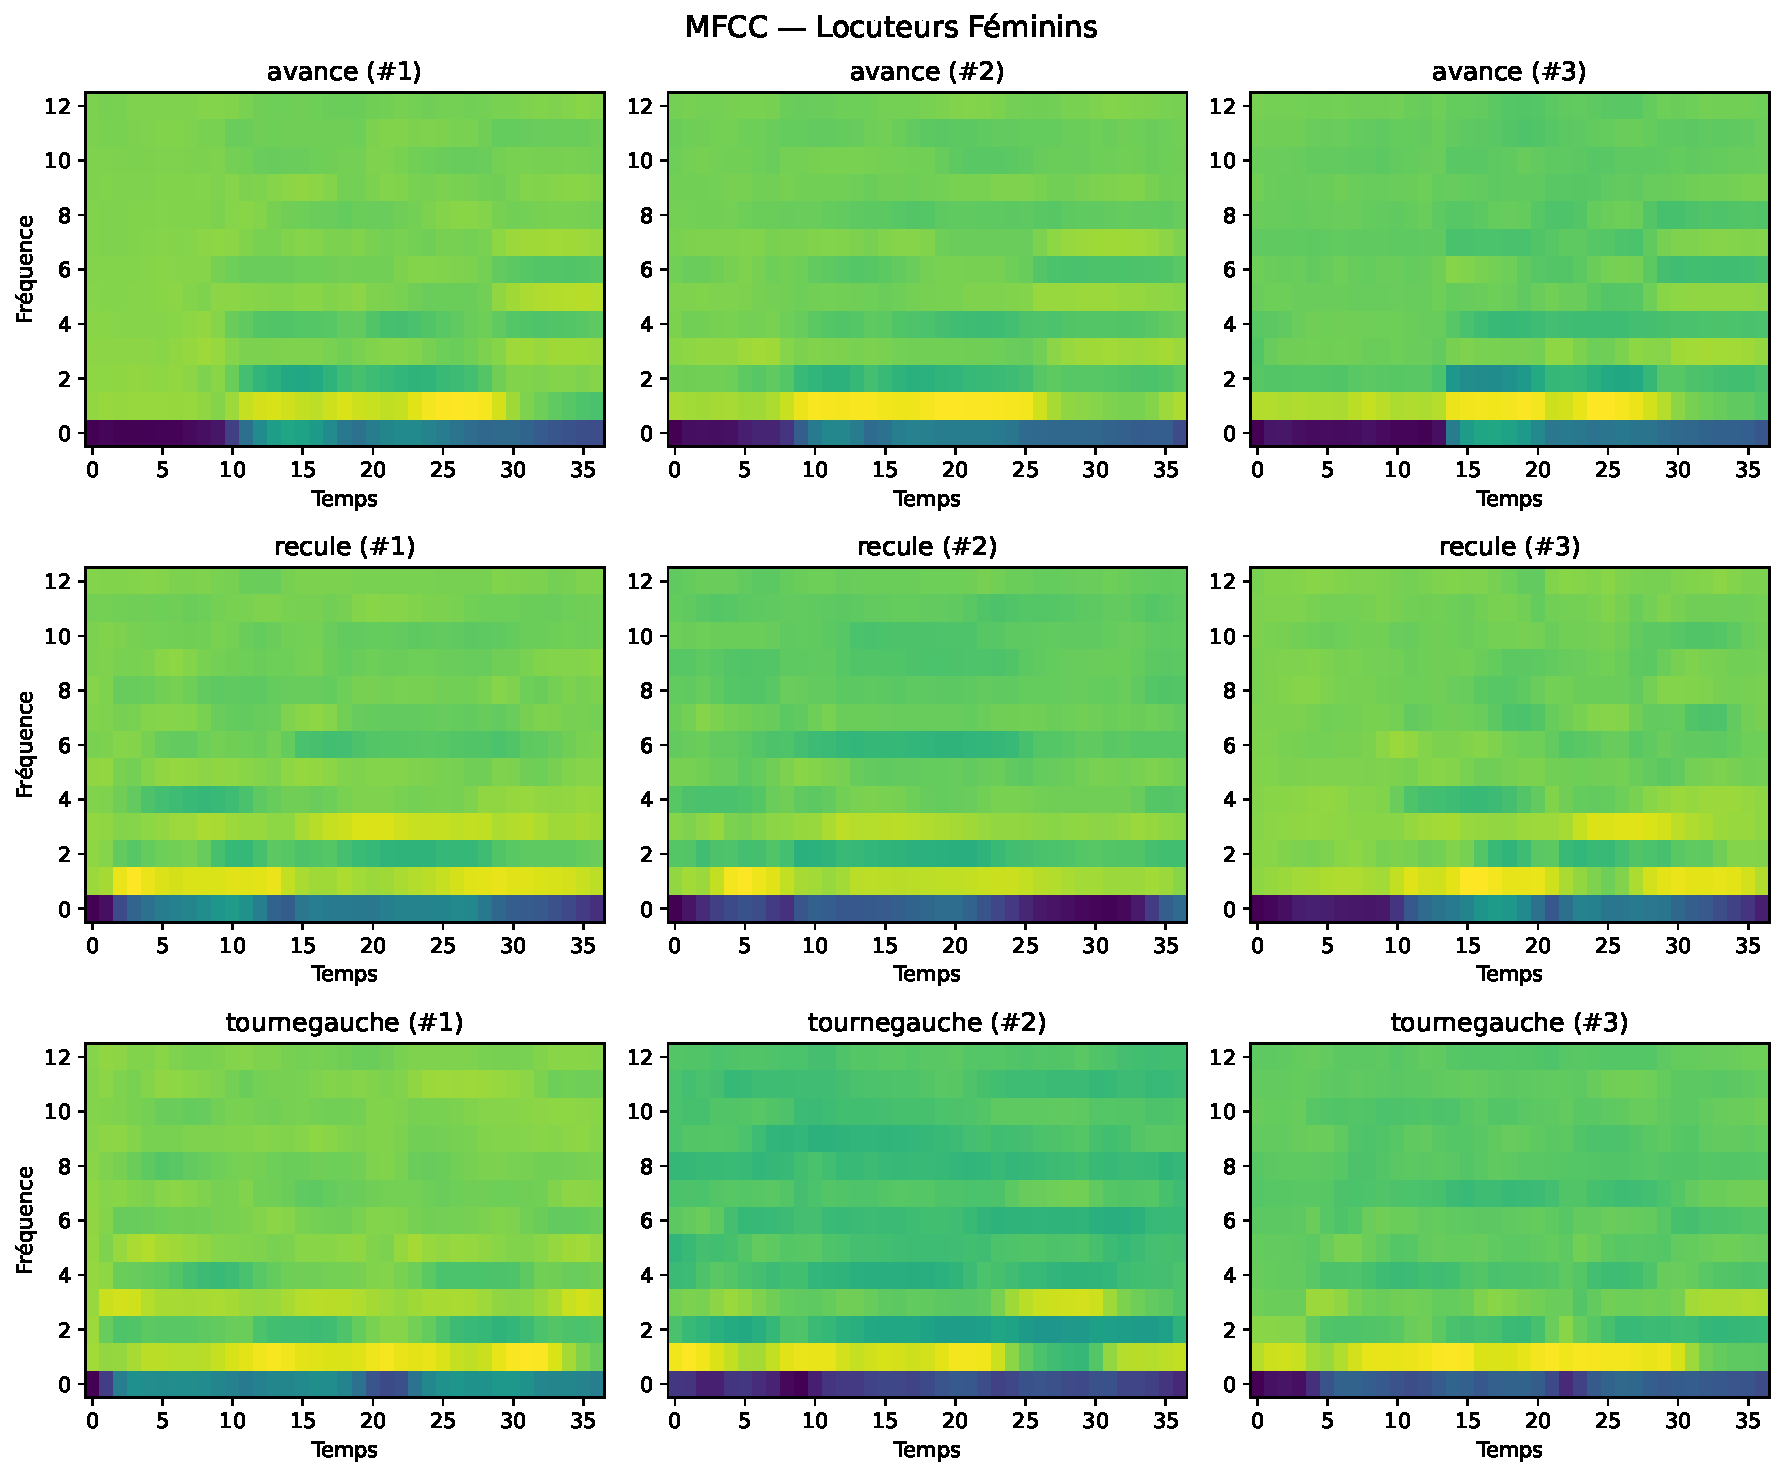
\includegraphics[width=\textwidth]{figures/mfcc_spectrograms_female.pdf}
        \caption{Locuteurs féminins}
    \end{subfigure}
    \caption{Coefficients MFCC de trois instances de chaque mot. Les MFCC capturent des informations compactes sur le contenu spectral perçu, avec des patterns visuellement distincts entre les commandes.}
    \label{fig:mfcc_spectrograms}
\end{figure}

\subsection{Transformeurs scikit-learn}

Pour intégrer ces prétraitements dans des pipelines scikit-learn, nous créons des classes conformes à l'interface \texttt{BaseEstimator / TransformerMixin} :

\begin{lstlisting}[caption={Classe FFT compatible scikit-learn}]
class FFT(BaseEstimator, TransformerMixin):
    def __init__(self, idx_frequence_max=None):
        self.idx_frequence_max = idx_frequence_max
    def fit(self, X, y=None):
        return self
    def transform(self, X, y=None):
        return preprocess_fft(X, idx_frequence_max=self.idx_frequence_max)
\end{lstlisting}

\begin{lstlisting}[caption={Classe STFT compatible scikit-learn}]
class STFT(BaseEstimator, TransformerMixin):
    def __init__(self, stat="mean", idx_frequence_max=None):
        self.stat = stat
        self.idx_frequence_max = idx_frequence_max
    def fit(self, X, y=None):
        return self
    def transform(self, X, y=None):
        return preprocess_stft(X, stat=self.stat, 
                               idx_frequence_max=self.idx_frequence_max, fs=22050)
\end{lstlisting}

\begin{lstlisting}[caption={Classe MFCC compatible scikit-learn}]
class MFCC(BaseEstimator, TransformerMixin):
    def __init__(self, stat="mean", n_mfcc=13):
        self.stat = stat
        self.n_mfcc = n_mfcc
    def fit(self, X, y=None):
        return self
    def transform(self, X, y=None):
        return preprocess_mfcc(X, stat=self.stat, sr=22050, n_mfcc=self.n_mfcc)
\end{lstlisting}

\notebox{Des Parties I à IV, le prétraitement \textbf{FFT + PCA} sera exclusivement utilisé, conformément à la consigne du sujet.}

%% ================================================================
%% SECTION 3 : PARTIE I - RÉGRESSION LOGISTIQUE
%% ================================================================
\newpage
\section{Partie I : Régression logistique multiclasse}

\subsection{Modèle}

On modélise les probabilités a posteriori par le modèle \textit{softmax} :

$$
\mathbb{P}(Y_i = j \mid X_i) = \frac{\exp(-\beta_j^T X_i)}{1 + \sum_{\ell=1}^{K-1} \exp(-\beta_\ell^T X_i)}, \quad \forall j \in \{1, \dots, K-1\}
$$

avec $K=3$ classes dans notre cas.

\subsection{Séparation train/test}

On sépare le dataset en 80\% entraînement / 20\% test avec stratification pour conserver les proportions de chaque classe :

\begin{lstlisting}[caption={Split stratifié 80/20}]
X_abs = preprocess_fft(X)  # Magnitudes FFT

X_train_raw, X_test_raw, y_train, y_test = train_test_split(
    X_abs, y, test_size=0.20, random_state=RANDOM_SEED, stratify=y
)

# PCA sur le train uniquement
pca = PCA(n_components=20, random_state=RANDOM_SEED)
X_train = pca.fit_transform(X_train_raw)
X_test = pca.transform(X_test_raw)
# Train: 43 | Test: 11
\end{lstlisting}

\subsection{Validation croisée Leave-One-Out manuelle}

On effectue une validation LOO manuelle en ajustant la PCA \textbf{uniquement sur les folds d'entraînement} à chaque itération :

\begin{lstlisting}[caption={LOO manuelle via l'API}]
result = manual_loo_score(
    X_raw=X_train_raw, y=y_train,
    preprocessor=PCA,
    classifier="logistic_regression",
    preprocessor_params={"n_components": 20, "random_state": RANDOM_SEED},
    classifier_params={"C": 1.0, "max_iter": 1000},
    verbose=True
)
\end{lstlisting}

\subsubsection{Pourquoi ne pas prétraiter avant la validation croisée ?}

L'ACP est une méthode non supervisée qui dépend de la distribution globale des données. Si on appliquait l'ACP sur l'ensemble des données avant le split :

\begin{enumerate}
    \item Les axes principaux contiendraient des informations sur la distribution du pli de validation (censé être invisible).
    \item Cela introduirait une \textbf{fuite d'information} (\textit{data leakage}), biaisant positivement l'évaluation.
\end{enumerate}

En ajustant la PCA uniquement sur les folds d'entraînement, on s'assure d'une évaluation honnête et réaliste.

\subsection{Grid Search manuelle}

On recherche les meilleurs hyperparamètres par grid search sur la grille :

\begin{center}
\begin{tabular}{ll}
\toprule
\textbf{Paramètre} & \textbf{Valeurs testées} \\
\midrule
\texttt{idx\_frequence\_max} & 1\,000, 3\,000 \\
\texttt{n\_components} (PCA) & 5, 20 \\
$C$ (régularisation LR) & 0.1, 10.0 \\
\bottomrule
\end{tabular}
\end{center}

\begin{lstlisting}[caption={Grid search manuelle}]
for idx_freq in [1000, 3000]:
    X_sliced = X_train_raw[:, :idx_freq]
    for n_comp in [5, 20]:
        for C in [0.1, 10.0]:
            result = manual_loo_score(
                X_raw=X_sliced, y=y_train,
                preprocessor=PCA, classifier="logistic_regression",
                preprocessor_params={"n_components": n_comp},
                classifier_params={"C": C, "max_iter": 1000},
            )
\end{lstlisting}

\subsection{Pipeline et GridSearchCV}

On encapsule le prétraitement et le classifier dans un \texttt{Pipeline} scikit-learn avec \texttt{GridSearchCV} :

\begin{lstlisting}[caption={Pipeline FFT > PCA > LR avec GridSearchCV}]
pipeline = Pipeline([
    ('fft', FFT()),
    ('pca', PCA(random_state=RANDOM_SEED)),
    ('clf', LogisticRegression(max_iter=1000, random_state=RANDOM_SEED))
])

param_grid = {
    'fft__idx_frequence_max': [1000, 3000],
    'pca__n_components':      [5, 20],
    'clf__C':                 [0.1, 10.0]
}

grid_search = GridSearchCV(pipeline, param_grid, cv=LeaveOneOut(), 
                           scoring='accuracy', n_jobs=-1)
grid_search.fit(X_train_raw, y_train)
\end{lstlisting}

\subsection{Évaluation des résultats}

\begin{figure}[H]
    \centering
    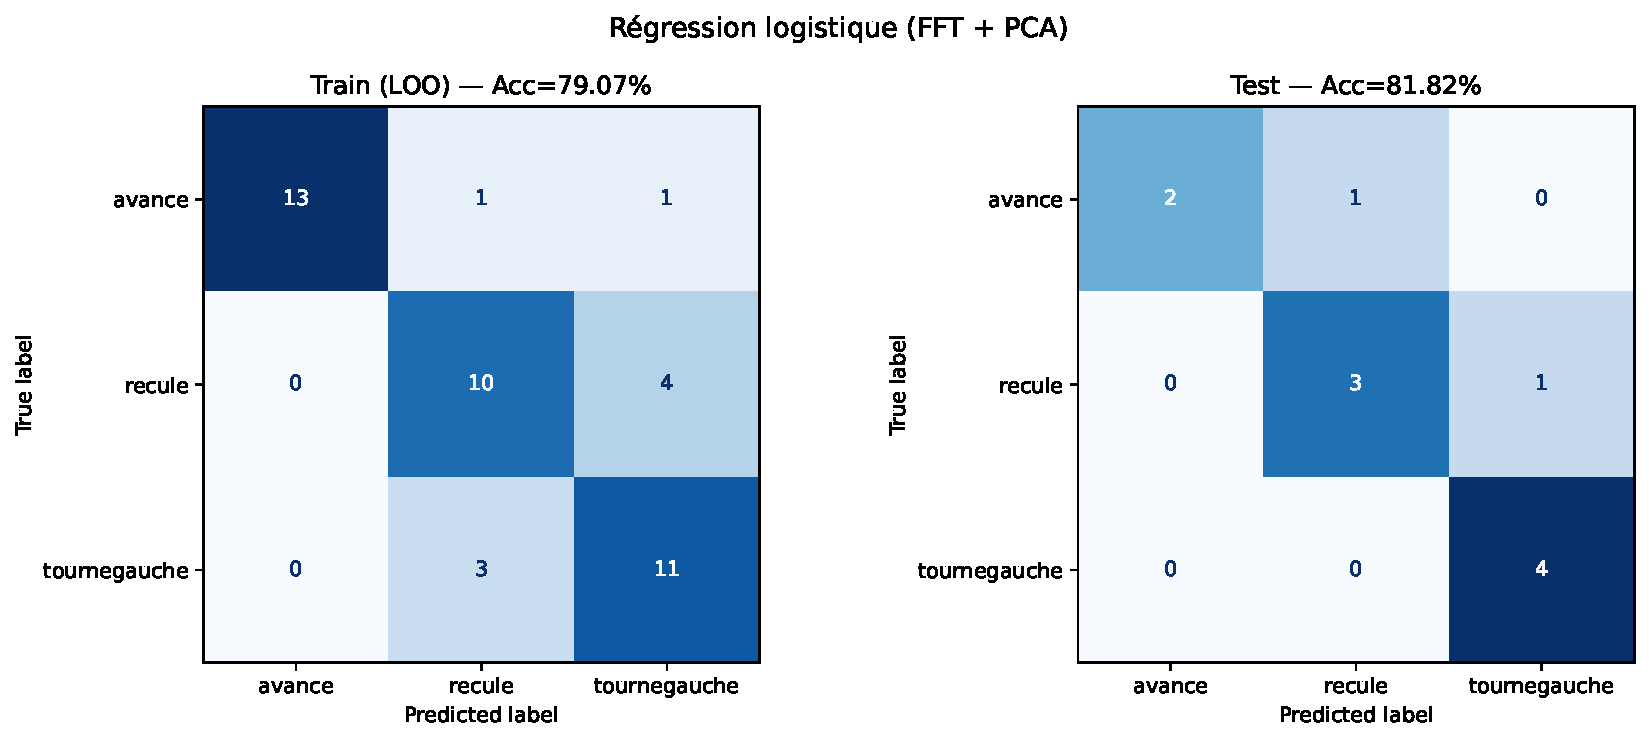
\includegraphics[width=0.95\textwidth]{figures/cm_logistic_regression.pdf}
    \caption{Matrices de confusion de la régression logistique (FFT + PCA) : à gauche les prédictions LOO sur le train, à droite sur le test. On observe que le modèle confond principalement \textit{recule} et \textit{tournegauche}.}
    \label{fig:cm_lr}
\end{figure}

\subsection{Impact du StandardScaler}

On ajoute un \texttt{StandardScaler} après l'ACP dans le pipeline :

\begin{lstlisting}[caption={Pipeline avec StandardScaler}]
pipeline_scaled = Pipeline([
    ('fft', FFT()),
    ('pca', PCA(random_state=RANDOM_SEED)),
    ('scaler', StandardScaler()),
    ('clf', LogisticRegression(max_iter=1000, random_state=RANDOM_SEED))
])
\end{lstlisting}

\begin{figure}[H]
    \centering
    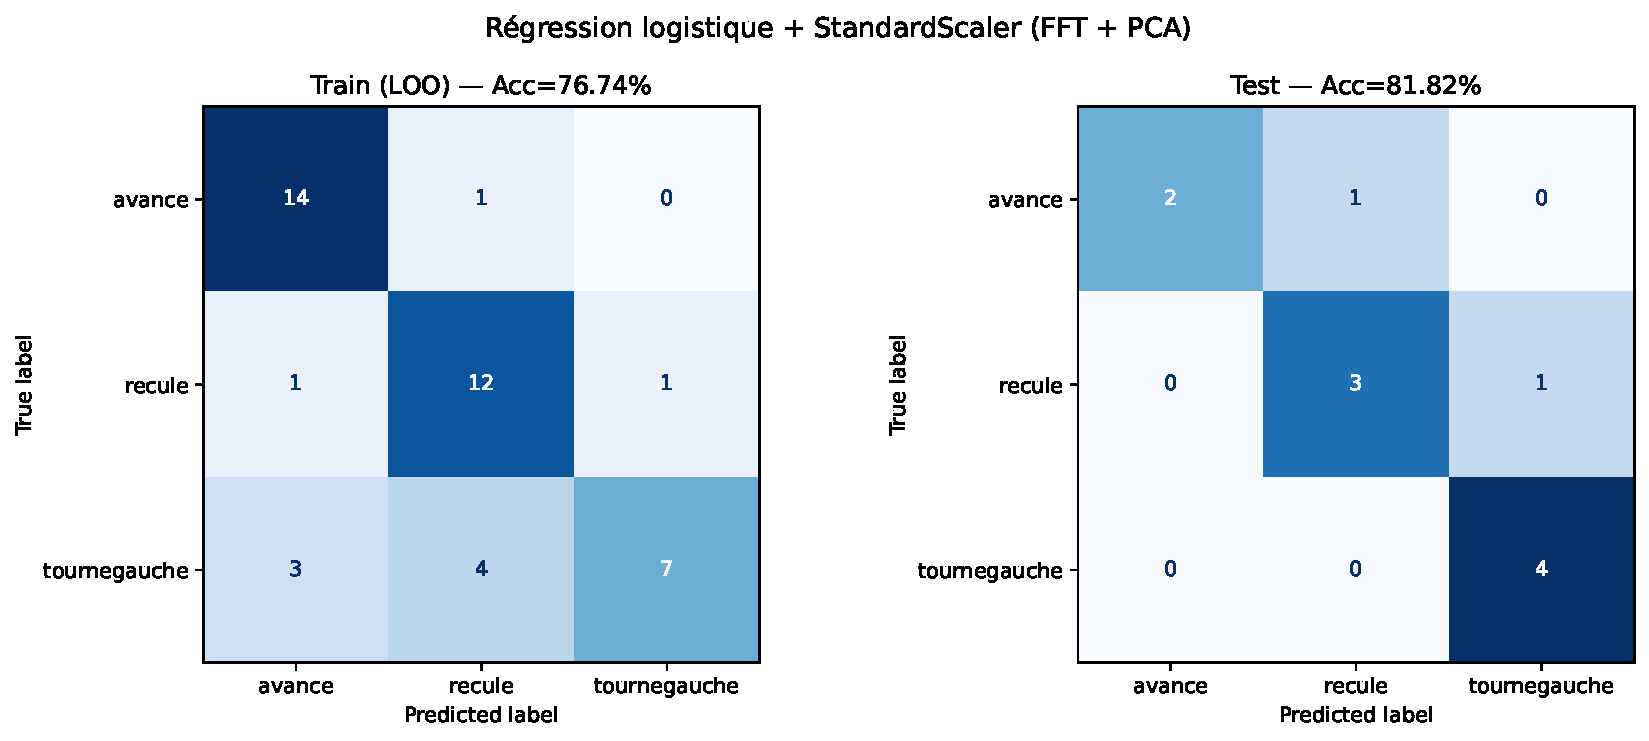
\includegraphics[width=0.95\textwidth]{figures/cm_logistic_regression_scaled.pdf}
    \caption{Matrices de confusion avec StandardScaler ajouté. La normalisation des features après ACP peut modifier les performances en mettant toutes les composantes à la même échelle, ce qui influence la régularisation $L_2$ implicite de la régression logistique.}
    \label{fig:cm_lr_scaled}
\end{figure}

%% ================================================================
%% SECTION 4 : PARTIE II - SVM
%% ================================================================
\newpage
\section{Partie II : Classification par méthodes à noyau}

\subsection{Rappel théorique}

Les méthodes à noyau consistent à projeter les données dans un espace de Hilbert $\mathcal{H}$ de dimension potentiellement infinie où les données deviennent linéairement séparables.

\begin{theorem}[Théorème de représentation]
La solution du problème de séparation dans $\mathcal{H}$ est contenue dans un sous-espace vectoriel de dimension finie de $\mathcal{H}$, engendré par les images des points d'entraînement.
\end{theorem}

Cela rend le problème calculable malgré la dimension infinie de $\mathcal{H}$, via l'\textit{astuce du noyau} (\textit{kernel trick}).

\subsection{SVM avec noyau RBF}

On utilise un pipeline complet \texttt{FFT $\to$ PCA $\to$ StandardScaler $\to$ SVM RBF} :

\begin{lstlisting}[caption={Pipeline SVM RBF}]
pipeline_svm = Pipeline([
    ('fft', FFT()),
    ('pca', PCA(random_state=RANDOM_SEED)),
    ('scaler', StandardScaler()),
    ('clf', SVC(kernel='rbf', random_state=RANDOM_SEED))
])

param_grid_svm = {
    'fft__idx_frequence_max': [1000, 3000],
    'pca__n_components':      [10, 20],
    'clf__C':                 [0.1, 10.0],
    'clf__gamma':             [0.001, 'scale']
}

grid_search_svm = GridSearchCV(pipeline_svm, param_grid_svm, 
                               cv=LeaveOneOut(), scoring='accuracy', n_jobs=-1)
grid_search_svm.fit(X_train_raw, y_train)
\end{lstlisting}

\subsection{Résultats et interprétation}

\begin{figure}[H]
    \centering
    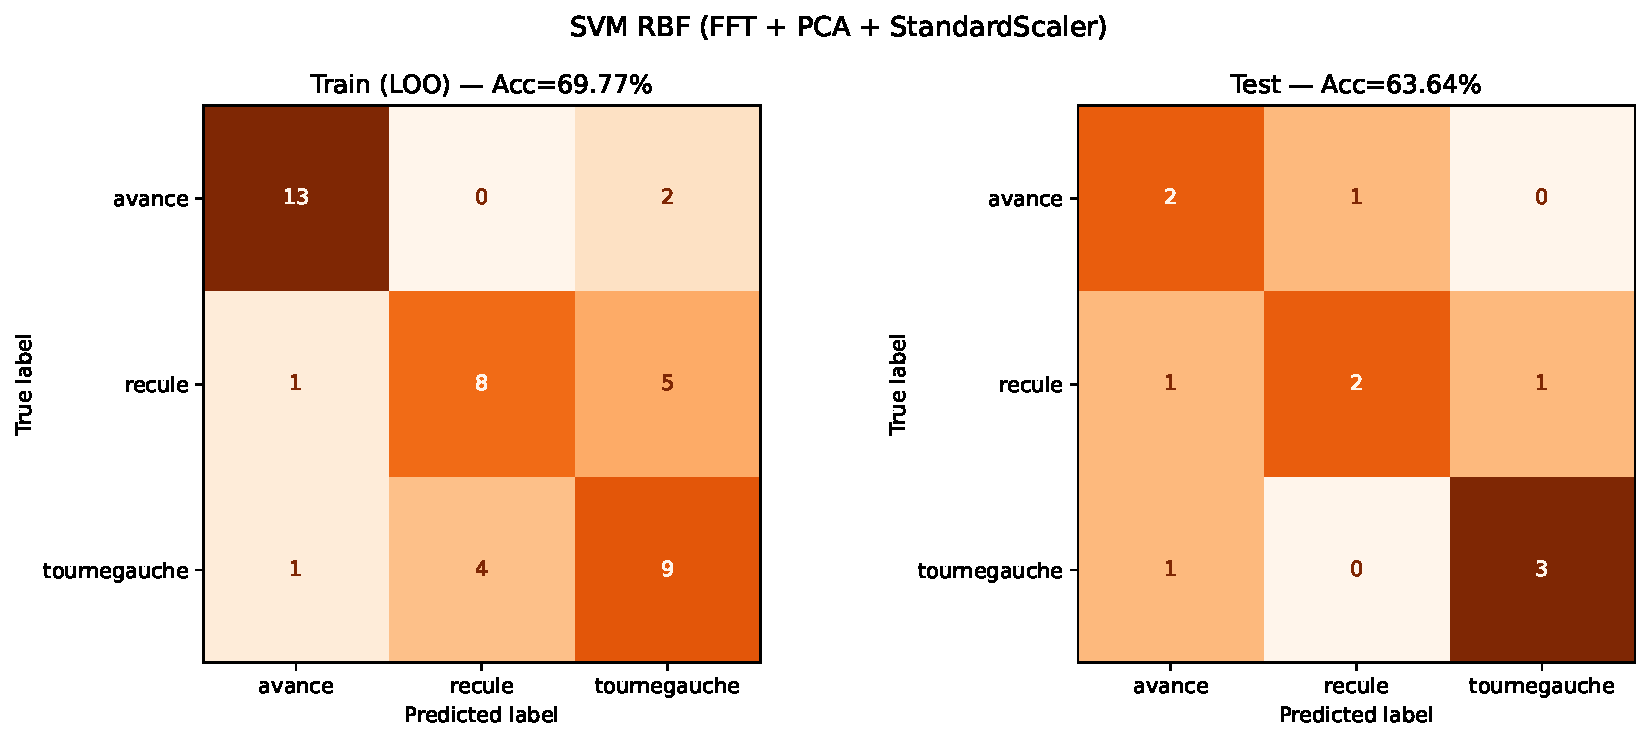
\includegraphics[width=0.95\textwidth]{figures/cm_svm_rbf.pdf}
    \caption{Matrices de confusion du SVM RBF. Le modèle est globalement performant sur le train (LOO) mais montre une baisse de précision sur le test set, suggérant du surapprentissage. La confusion entre \textit{recule} et \textit{tournegauche} persiste, reflétant la proximité spectrale de ces commandes.}
    \label{fig:cm_svm}
\end{figure}

Le SVM avec noyau RBF capture des frontières de décision non linéaires, mais sur un dataset aussi petit (43 exemples d'entraînement), le risque de surapprentissage est élevé. La baisse de performances entre le score LOO et le score test confirme cette sensibilité.

%% ================================================================
%% SECTION 5 : PARTIE III - MÉTHODES D'ENSEMBLE
%% ================================================================
\newpage
\section{Partie III : Méthodes d'ensemble}

Pour cette partie, on passe en classification binaire : $y^1 = 1$ si $y = 1$ (\textit{recule}), $y^1 = 0$ sinon. Le prétraitement reste FFT + PCA (20 composantes).

\subsection{Bootstrap Aggregation (Bagging)}

Le Bagging consiste à créer $M$ jeux de données bootstrap (tirage avec remise de $N$ points parmi $N$), entraîner un classifieur faible sur chacun, puis agréger les prédictions par vote majoritaire.

\begin{lstlisting}[caption={Bagging from scratch via l'API}]
from projet_fil_rouge.classifiers.ensembles.bagging import BaggingClassifier

bag_scratch = BaggingClassifier(
    base_classifier=DecisionTreeClassifier(max_depth=2, random_state=RANDOM_SEED),
    n_estimators=100, random_state=RANDOM_SEED
)
bag_scratch.fit(X_train_bag, y_train_bag)
y_pred_bagging = bag_scratch.predict(X_test_bag)
\end{lstlisting}

\subsection{Random Forest}

La Random Forest est une variante du Bagging qui ajoute du \textit{feature bagging} : à chaque nœud de chaque arbre, seul un sous-ensemble aléatoire de features est considéré pour la coupe. Cela réduit la corrélation entre les arbres et améliore la diversité de l'ensemble.

\begin{lstlisting}[caption={Random Forest sklearn}]
rf_model = RandomForestClassifier(n_estimators=100, max_depth=2, random_state=RANDOM_SEED)
rf_model.fit(X_train_bag, y_train_bag)
\end{lstlisting}

\begin{figure}[H]
    \centering
    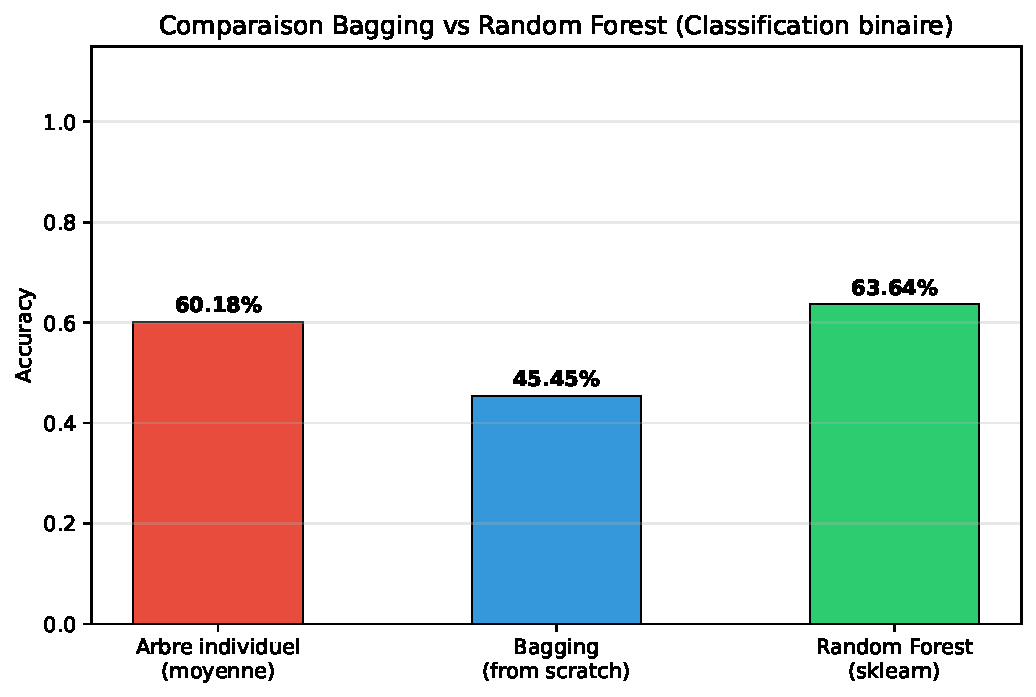
\includegraphics[width=0.85\textwidth]{figures/bagging_rf_comparison.pdf}
    \caption{Comparaison Bagging vs Random Forest. Le Bagging améliore significativement la précision par rapport aux arbres individuels (réduction de variance). La Random Forest obtient des performances comparables avec l'avantage supplémentaire de la décorrélation des arbres.}
    \label{fig:bagging_rf}
\end{figure}

\subsection{AdaBoost (Adaptive Boosting)}

Contrairement au Bagging qui combine des modèles indépendants, AdaBoost construit séquentiellement des classifieurs en pondérant les exemples difficiles.

\textbf{Algorithme :}
\begin{enumerate}
    \item Initialiser $w_n^{(1)} = 1/N$ pour $n = 1, \dots, N$
    \item Pour $m = 1, \dots, M$ :
    \begin{enumerate}
        \item Entraîner $y_m(x)$ en minimisant $J_m = \sum_{n=1}^N w_n^{(m)} \mathbb{1}(y_m(x_n) \neq t_n)$
        \item Calculer $\epsilon_m = \frac{\sum_{n=1}^N w_n^{(m)} \mathbb{1}(y_m(x_n) \neq t_n)}{\sum_{n=1}^N w_n^{(m)}}$ \quad puis \quad $\alpha_m = \ln\left(\frac{1 - \epsilon_m}{\epsilon_m}\right)$
        \item Mettre à jour $w_n^{(m+1)} = w_n^{(m)} \exp\left(\alpha_m \mathbb{1}(y_m(x_n) \neq t_n)\right)$
    \end{enumerate}
    \item Prédire : $Y_M(x) = \text{sign}\left(\sum_{m=1}^M \alpha_m y_m(x)\right)$
\end{enumerate}

\begin{lstlisting}[caption={AdaBoost from scratch via l'API}]
from projet_fil_rouge.classifiers.ensembles.adaboost import ScratchAdaBoostClassifier

ada_scratch = ScratchAdaBoostClassifier(
    base_classifier=DecisionTreeClassifier(max_depth=2, random_state=RANDOM_SEED),
    n_estimators=100, random_state=RANDOM_SEED
)
ada_scratch.fit(X_train_bag, y_train_bag)
\end{lstlisting}

\subsection{AdaBoost et Gradient Boosting (sklearn)}

On utilise les implémentations sklearn avec \texttt{GridSearchCV} en LOO :

\begin{lstlisting}[caption={AdaBoost et Gradient Boosting sklearn avec GridSearchCV}]
# AdaBoost
ada_clf = AdaBoostClassifier(
    estimator=DecisionTreeClassifier(max_depth=2), random_state=RANDOM_SEED
)
grid_ada = GridSearchCV(ada_clf, 
    {'n_estimators': [50, 100], 'learning_rate': [0.1, 1.0]},
    cv=LeaveOneOut(), scoring='accuracy', n_jobs=-1)
grid_ada.fit(X_train_bag, y_train_bag)

# Gradient Boosting
gb_clf = GradientBoostingClassifier(max_depth=2, random_state=RANDOM_SEED)
grid_gb = GridSearchCV(gb_clf,
    {'n_estimators': [50, 100], 'learning_rate': [0.01, 0.1]},
    cv=LeaveOneOut(), scoring='accuracy', n_jobs=-1)
grid_gb.fit(X_train_bag, y_train_bag)
\end{lstlisting}

\begin{figure}[H]
    \centering
    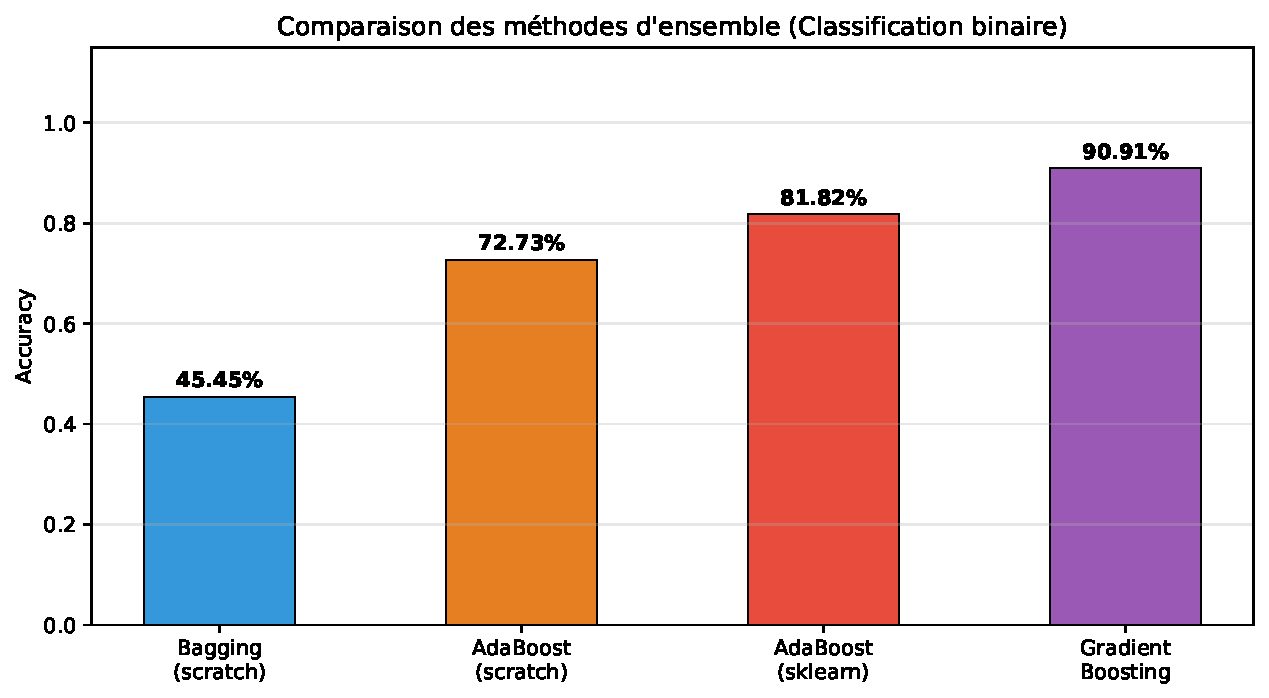
\includegraphics[width=0.9\textwidth]{figures/ensemble_comparison.pdf}
    \caption{Comparaison de toutes les méthodes d'ensemble sur la classification binaire. Le Gradient Boosting et l'AdaBoost montrent l'intérêt du boosting séquentiel face au bagging parallèle, bien que les différences soient limitées sur un dataset aussi petit.}
    \label{fig:ensemble_comparison}
\end{figure}

%% ================================================================
%% SECTION 6 : PARTIE IV - RÉSEAUX DE NEURONES
%% ================================================================
\newpage
\section{Partie IV : Réseaux de neurones avec PyTorch}

\subsection{Préparation des données}

On applique le prétraitement FFT + PCA (20 composantes), puis on convertit en tenseurs PyTorch de forme $(N, B, F)$ avec $B=1$ (batch unitaire) et $F=20$ features. Le split est 50/50 conformément à la consigne.

\begin{lstlisting}[caption={Préparation des tenseurs PyTorch}]
import torch

X_preprocessed = PCA(n_components=20).fit_transform(preprocess_fft(X))
X_train, X_test, y_train, y_test = train_test_split(
    X_preprocessed, y, test_size=0.5, random_state=RANDOM_SEED, stratify=y
)

X_train = torch.tensor(X_train).reshape((N_train, 1, -1)).float()
X_test  = torch.tensor(X_test).reshape((N_test, 1, -1)).float()
y_train = F.one_hot(torch.tensor(y_train), num_classes=3).reshape((N_train, 1, -1)).float()
y_test  = F.one_hot(torch.tensor(y_test), num_classes=3).reshape((N_test, 1, -1)).float()
\end{lstlisting}

\subsection{Question 1 : Architecture reproduisant la régression logistique}

Pour reproduire une régression logistique multiclasse, on utilise une seule couche linéaire sans activation (les logits sont directement passés à la \texttt{CrossEntropyLoss} qui applique le softmax) :

\begin{lstlisting}[caption={Modèle PyTorch reproduisant la régression logistique}]
class NNClassification(torch.nn.Module):
    def __init__(self):
        super().__init__()
        self.network = torch.nn.Sequential(
            nn.Linear(20, 3)  # 20 features -> 3 classes
        )
    
    def forward(self, xb):
        return self.network(xb)
\end{lstlisting}

La \textbf{CrossEntropyLoss} est naturellement adaptée : elle combine \texttt{LogSoftmax} et \texttt{NLLLoss}, ce qui est exactement l'objectif d'optimisation de la régression logistique multiclasse.

\subsection{Question 2 : Boucle d'entraînement et courbes de perte}

\begin{lstlisting}[caption={Boucle d'entraînement PyTorch}]
model = NNClassification()
optimizer = torch.optim.Adam(model.parameters(), lr=0.01)
loss_fn = nn.CrossEntropyLoss()

for epoch in range(15):
    model.train()
    for i in range(X_train.shape[0]):
        optimizer.zero_grad()
        pred = model(X_train[i])
        target_idx = torch.argmax(y_train[i], dim=-1)
        loss = loss_fn(pred, target_idx)
        loss.backward()
        optimizer.step()
    
    model.eval()
    with torch.no_grad():
        # Calcul de la loss sur le test set
        ...
\end{lstlisting}

\begin{figure}[H]
    \centering
    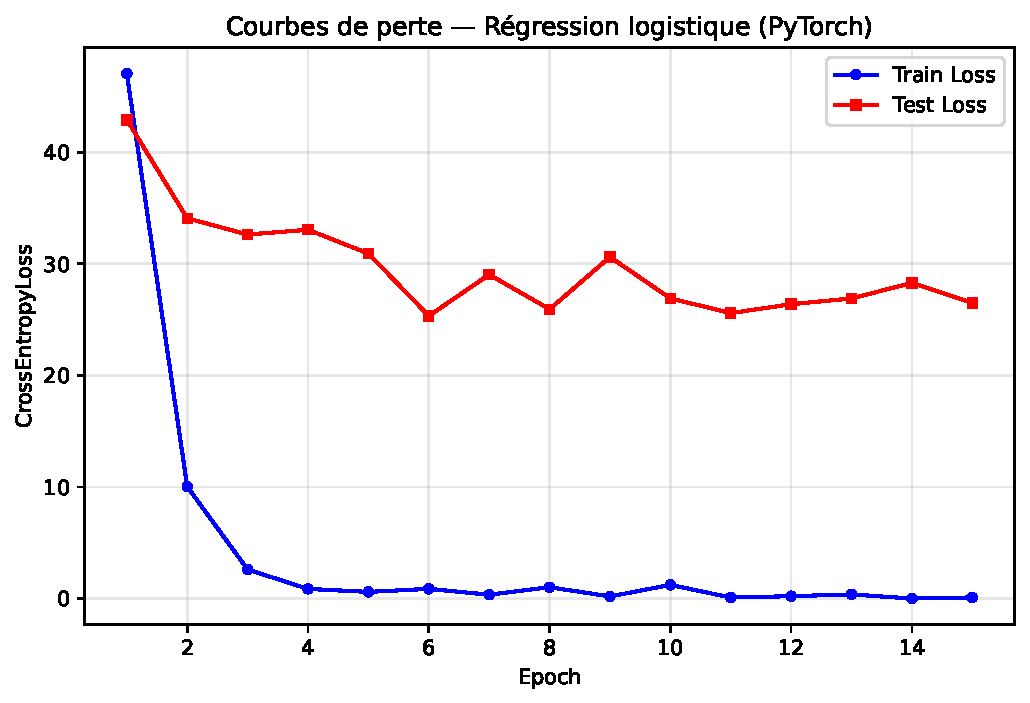
\includegraphics[width=0.8\textwidth]{figures/nn_loss_curves.pdf}
    \caption{Évolution des pertes d'entraînement et de test. On observe une convergence rapide (dès les premières epochs) typique d'un modèle linéaire sur un très petit dataset. Les pertes train et test évoluent de manière similaire, signe que le modèle ne sur-apprend pas significativement.}
    \label{fig:nn_loss}
\end{figure}

\subsection{Question 3 : Accuracy et matrice de confusion}

\begin{figure}[H]
    \centering
    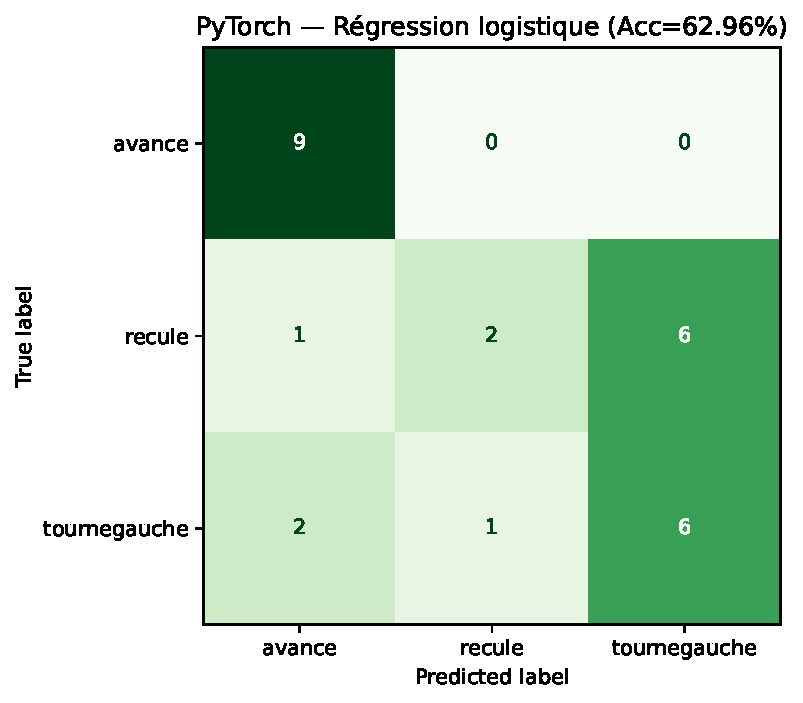
\includegraphics[width=0.55\textwidth]{figures/cm_nn_logistic.pdf}
    \caption{Matrice de confusion du modèle PyTorch (régression logistique) sur le jeu de test.}
    \label{fig:cm_nn}
\end{figure}

\subsection{Question 4 : Régularisation (Dropout + L2)}

Pour combattre le surapprentissage potentiel, on ajoute :
\begin{itemize}
    \item Une couche cachée de 64 neurones avec ReLU
    \item Du \textbf{Dropout} (taux 0.3) après l'activation
    \item Une régularisation \textbf{L2} via \texttt{weight\_decay} dans l'optimiseur Adam
\end{itemize}

\begin{lstlisting}[caption={FNN régularisé avec Dropout et L2}]
class RegularizedNN(torch.nn.Module):
    def __init__(self, dropout_rate=0.3):
        super().__init__()
        self.network = torch.nn.Sequential(
            nn.Linear(20, 64),
            nn.ReLU(),
            nn.Dropout(dropout_rate),
            nn.Linear(64, 3)
        )

optimizer = torch.optim.Adam(model.parameters(), lr=0.005, weight_decay=1e-3)
\end{lstlisting}

\begin{figure}[H]
    \centering
    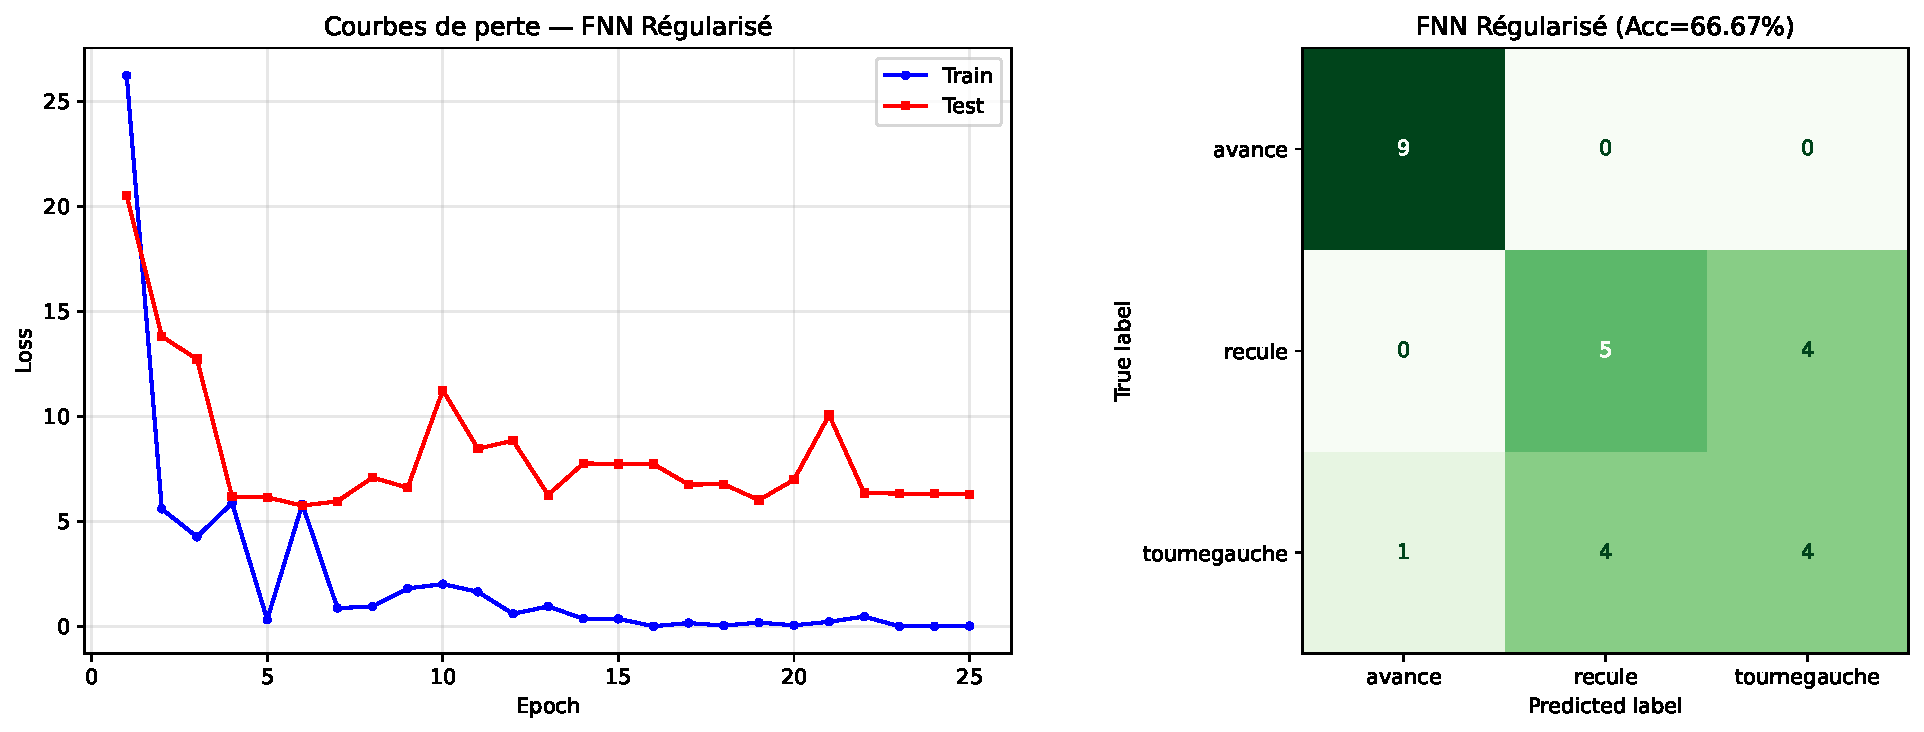
\includegraphics[width=0.95\textwidth]{figures/nn_regularized.pdf}
    \caption{Résultats du FNN régularisé : courbes de perte (gauche) et matrice de confusion (droite). La régularisation stabilise l'entraînement et peut améliorer la généralisation, bien que sur 27 exemples de test, les variations stochastiques dominent.}
    \label{fig:nn_reg}
\end{figure}

\subsection{Question 5 (Bonus) : CNN 1D sur signaux bruts}

On conçoit un CNN 1D qui prend directement le signal acoustique brut en entrée (sans prétraitement) :

\begin{lstlisting}[caption={Architecture CNN 1D sur signaux bruts}]
class AudioCNN1D(torch.nn.Module):
    def __init__(self):
        super().__init__()
        self.conv = torch.nn.Sequential(
            nn.Conv1d(in_channels=1, out_channels=8, kernel_size=15, stride=4),
            nn.ReLU(),
            nn.MaxPool1d(kernel_size=4),
            nn.Conv1d(in_channels=8, out_channels=16, kernel_size=7, stride=2),
            nn.ReLU(),
            nn.MaxPool1d(kernel_size=4),
            nn.Flatten()
        )
        # Calcul dynamique de la taille de sortie
        with torch.no_grad():
            flat_size = self.conv(torch.zeros(1, 1, 18522)).shape[1]
        self.fc = nn.Sequential(
            nn.Linear(flat_size, 64), nn.ReLU(), nn.Linear(64, 3)
        )
    
    def forward(self, x):
        return self.fc(self.conv(x))
\end{lstlisting}

L'avantage de cette approche est que le CNN peut \textbf{apprendre ses propres features spectrales} directement à partir du signal brut, sans dépendre d'un choix a priori de prétraitement (FFT, MFCC, etc.).

\begin{figure}[H]
    \centering
    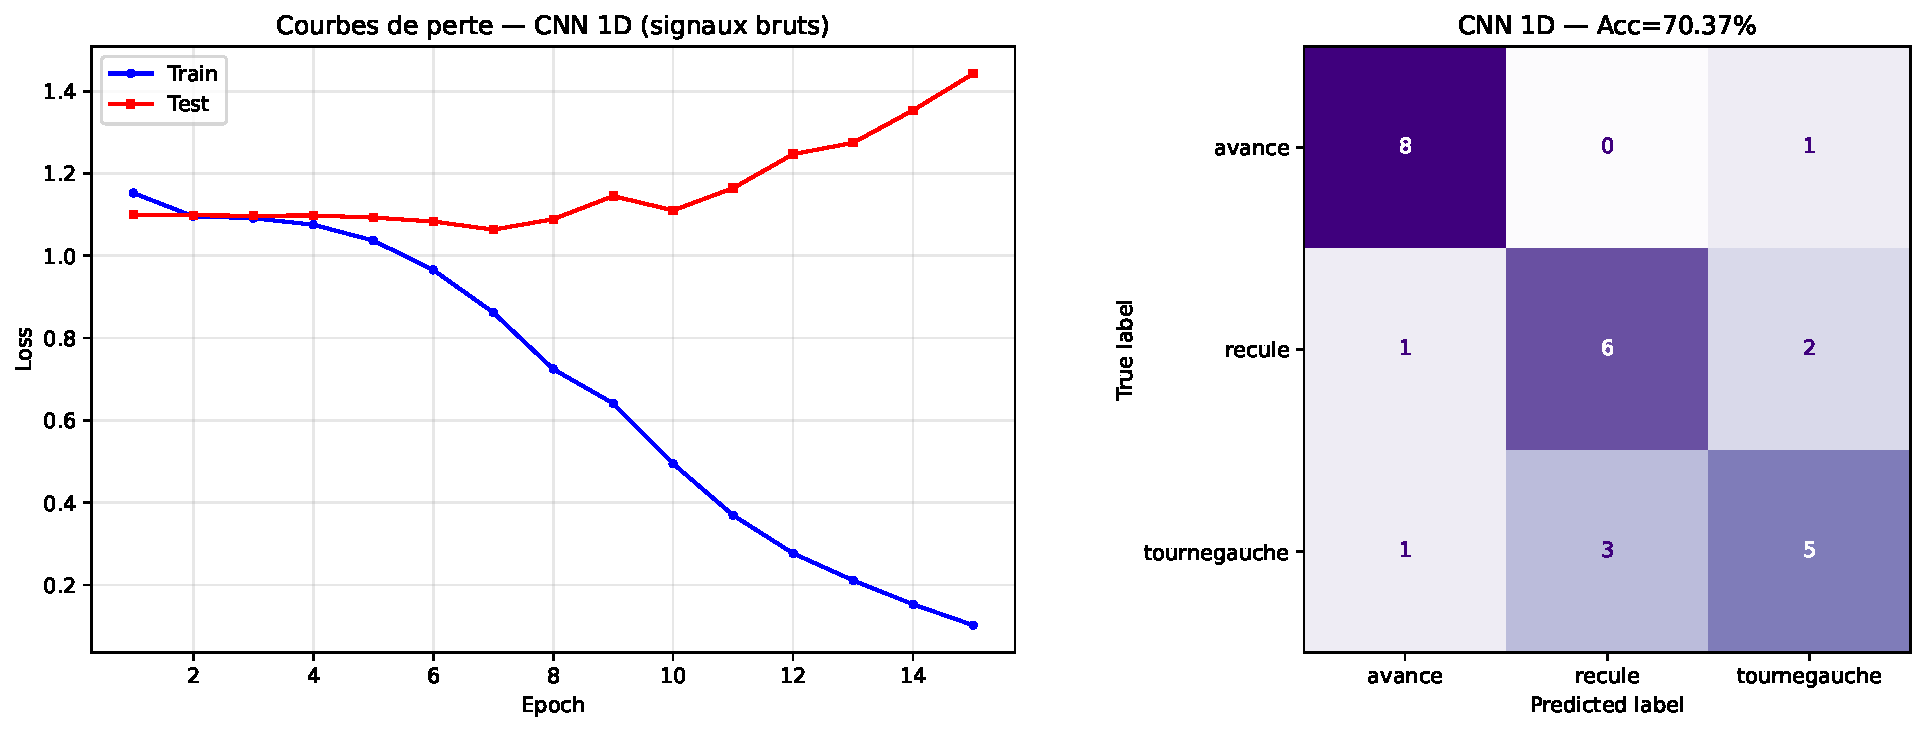
\includegraphics[width=0.95\textwidth]{figures/cnn_1d_results.pdf}
    \caption{Résultats du CNN 1D sur signaux bruts. À gauche : courbes de perte (convergence plus lente que le modèle linéaire). À droite : matrice de confusion sur le test. Le CNN apprend des représentations directement depuis le signal audio, démontrant la faisabilité de l'approche end-to-end.}
    \label{fig:cnn_results}
\end{figure}

%% ================================================================
%% SECTION 7 : PARTIE V - NOTRE ÉTUDE
%% ================================================================
\newpage
\section{Partie V : Notre Étude}

\subsection{Objectifs et méthodologie}

Notre étude personnelle consiste en un \textbf{benchmark exhaustif} visant à comparer systématiquement toutes les combinaisons possibles de méthodes de prétraitement, de classifiers et de méthodes d'évaluation.

L'objectif est double :
\begin{enumerate}
    \item Déterminer quelle méthode de prétraitement est la plus discriminante pour la reconnaissance de commandes audio
    \item Identifier les classifiers les plus robustes et les meilleures combinaisons prétraitement $\times$ classifier
\end{enumerate}

\subsubsection{Architecture du benchmark}

Le benchmark croise systématiquement :

\begin{center}
\begin{tabular}{lll}
\toprule
\textbf{Dimension} & \textbf{Nombre} & \textbf{Détail} \\
\midrule
Preprocessors & 9 & FFT+PCA, FFT+Kernel PCA, FFT+LDA, FFT+NMF, \\
 & & FFT+SVD, STFT, MFCC, MFCC Summary, Wavelet \\
Classifiers & 10 & LR, SVM, NN, Bagging (LR/SVM/NN/Tree), \\
 & & Random Forest, AdaBoost, Gradient Boosting \\
Fit methods & 3 & GridSearchCV, Train/Test, Manual LOO \\
\midrule
\textbf{Total} & \textbf{35\,668} & expériences (avec grilles d'hyperparamètres) \\
\bottomrule
\end{tabular}
\end{center}

Chaque expérience teste une combinaison spécifique d'hyperparamètres pour le preprocessor et le classifier, évaluée par la méthode de fit choisie. Le benchmark a été orchestré par notre librairie (\texttt{part5\_benchmark\_aggressive.py}).

\subsection{Comparaison des méthodes de prétraitement}

\begin{figure}[H]
    \centering
    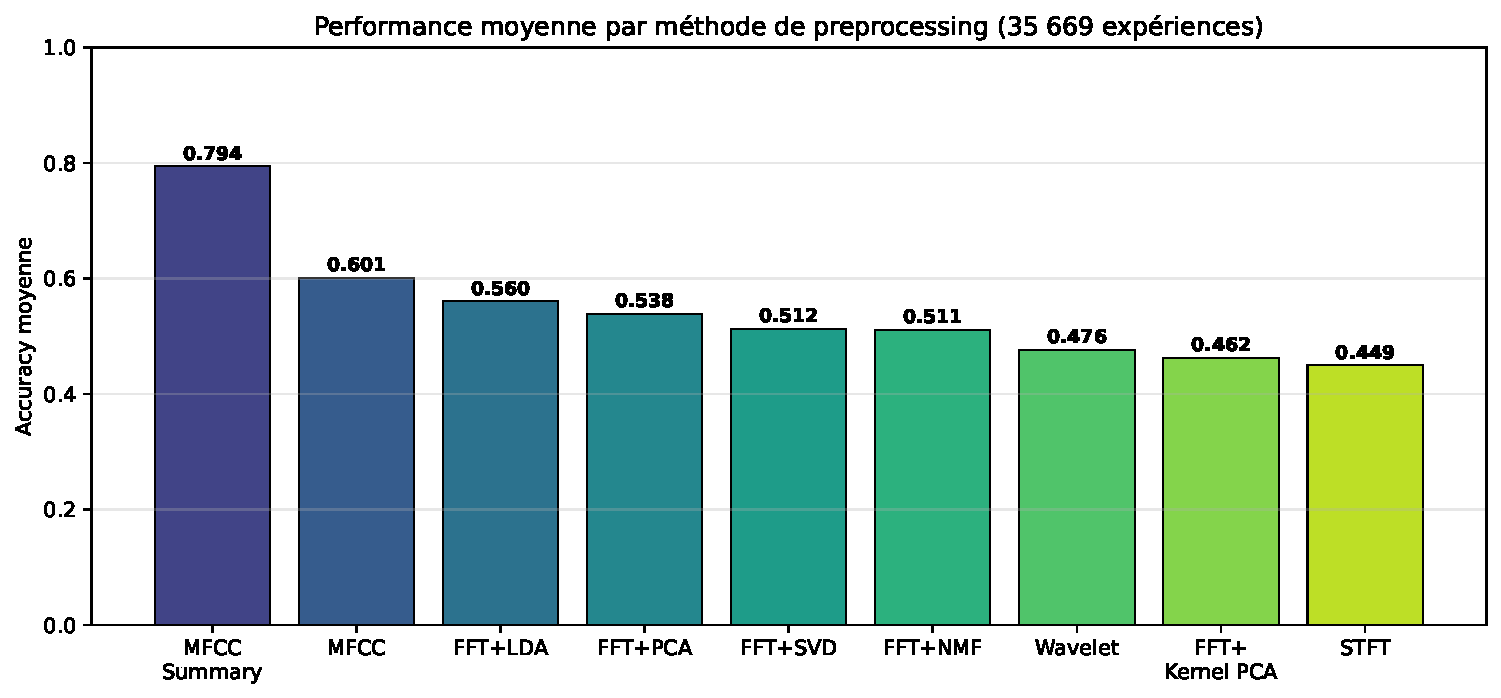
\includegraphics[width=0.95\textwidth]{figures/benchmark_by_preprocessor.pdf}
    \caption{Performance moyenne par méthode de preprocessing, agrégée sur tous les classifiers et méthodes d'évaluation.}
    \label{fig:bench_prep}
\end{figure}

\begin{center}
\begin{tabular}{clccc}
\toprule
\textbf{Rang} & \textbf{Preprocessor} & \textbf{N runs} & \textbf{Acc. moy.} & \textbf{Acc. max} \\
\midrule
1 & \textbf{MFCC Summary} & 1\,234 & \textbf{0.794} & 1.000 \\
2 & MFCC (stats) & 1\,798 & 0.601 & 1.000 \\
3 & FFT + LDA & 904 & 0.560 & 0.909 \\
4 & FFT + PCA & 5\,182 & 0.538 & 1.000 \\
5 & FFT + SVD & 5\,182 & 0.512 & 0.909 \\
6 & FFT + NMF & 5\,182 & 0.511 & 0.909 \\
7 & Wavelet & 1\,608 & 0.476 & 1.000 \\
8 & FFT + Kernel PCA & 10\,354 & 0.462 & 0.909 \\
9 & STFT & 3\,442 & 0.449 & 1.000 \\
\bottomrule
\end{tabular}
\end{center}

\textbf{Analyse :} Le MFCC Summary domine massivement les autres méthodes (0.794 vs 0.601 pour le MFCC simple, soit +32\%). Cela s'explique par le fait que le MFCC Summary combine moyenne \textit{et} écart-type des coefficients cepstraux, capturant à la fois la tendance centrale et la variabilité temporelle du signal. Les méthodes basées sur FFT avec réduction linéaire (PCA, SVD, NMF) sont en retrait, suggérant que la représentation perceptuelle (échelle de Mel) est plus adaptée à la discrimination de commandes vocales que la représentation fréquentielle brute.

\subsection{Comparaison des classifiers}

\begin{figure}[H]
    \centering
    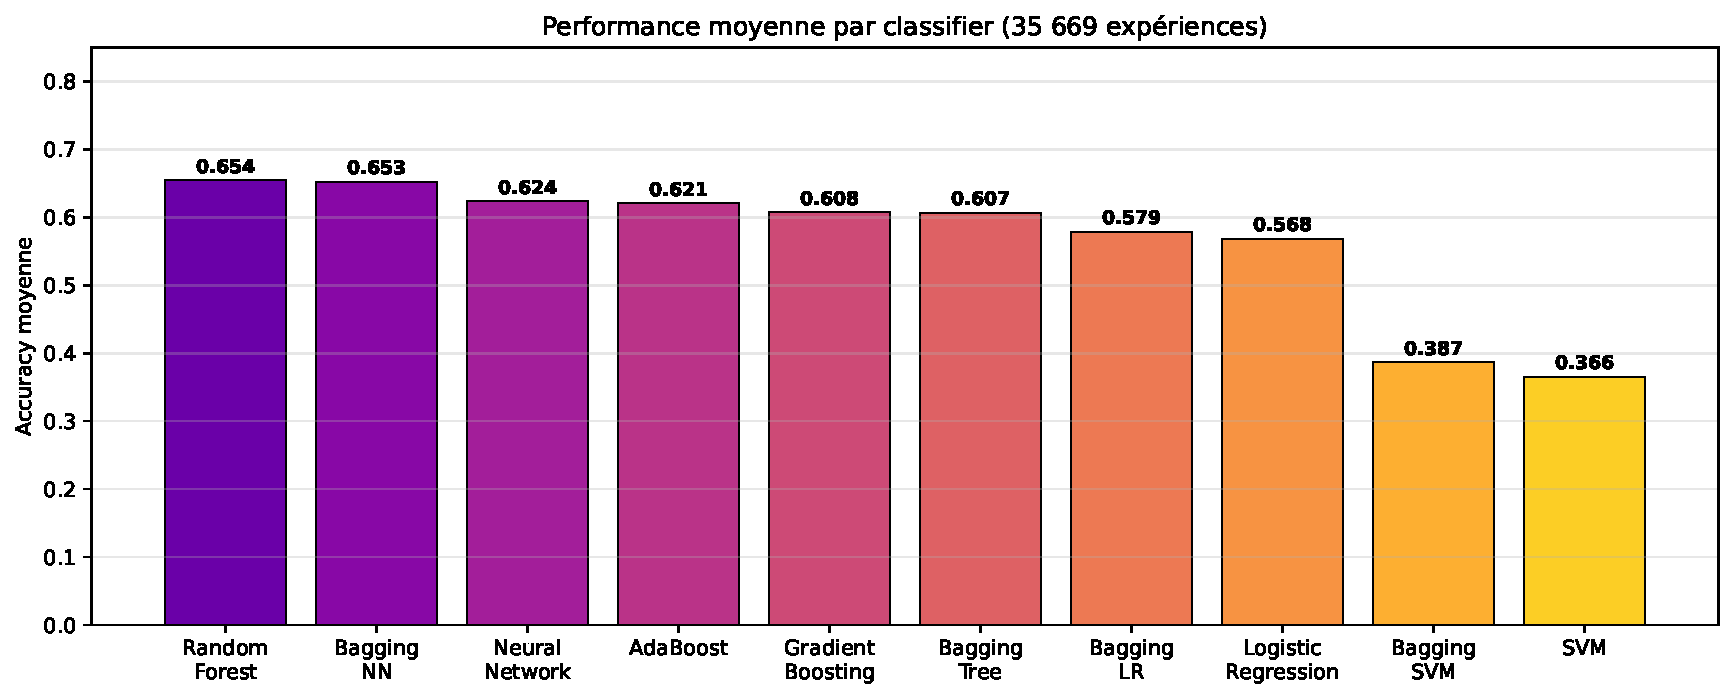
\includegraphics[width=0.95\textwidth]{figures/benchmark_by_classifier.pdf}
    \caption{Performance moyenne par classifier, agrégée sur tous les preprocessors et méthodes d'évaluation.}
    \label{fig:bench_clf}
\end{figure}

\begin{center}
\begin{tabular}{clccc}
\toprule
\textbf{Rang} & \textbf{Classifier} & \textbf{N runs} & \textbf{Acc. moy.} & \textbf{Acc. max} \\
\midrule
1 & \textbf{Random Forest} & 2\,833 & \textbf{0.654} & 1.000 \\
2 & Bagging NN & 873 & 0.653 & 1.000 \\
3 & Neural Network & 4\,197 & 0.624 & 1.000 \\
4 & AdaBoost & 2\,111 & 0.621 & 1.000 \\
5 & Gradient Boosting & 2\,111 & 0.608 & 1.000 \\
6 & Bagging Tree & 2\,127 & 0.607 & 1.000 \\
7 & Bagging LR & 3\,507 & 0.579 & 1.000 \\
8 & Logistic Regression & 1\,429 & 0.568 & 1.000 \\
9 & Bagging SVM & 11\,145 & 0.387 & 1.000 \\
10 & SVM & 4\,553 & 0.366 & 1.000 \\
\bottomrule
\end{tabular}
\end{center}

\textbf{Analyse :} La Random Forest et le Bagging NN sont les meilleurs classifiers en moyenne. Le SVM et le Bagging SVM sont en dernière position (0.37). Ce résultat surprenant s'explique par le fait que le SVM est très sensible à ses hyperparamètres ($C$, $\gamma$) : sur la grille large du benchmark, beaucoup de combinaisons sont sous-optimales. Avec un bon tuning (comme en Partie II avec GridSearchCV ciblé), le SVM peut obtenir de bons résultats localement.

\subsection{Analyse croisée : Preprocessing $\times$ Classifier}

\begin{figure}[H]
    \centering
    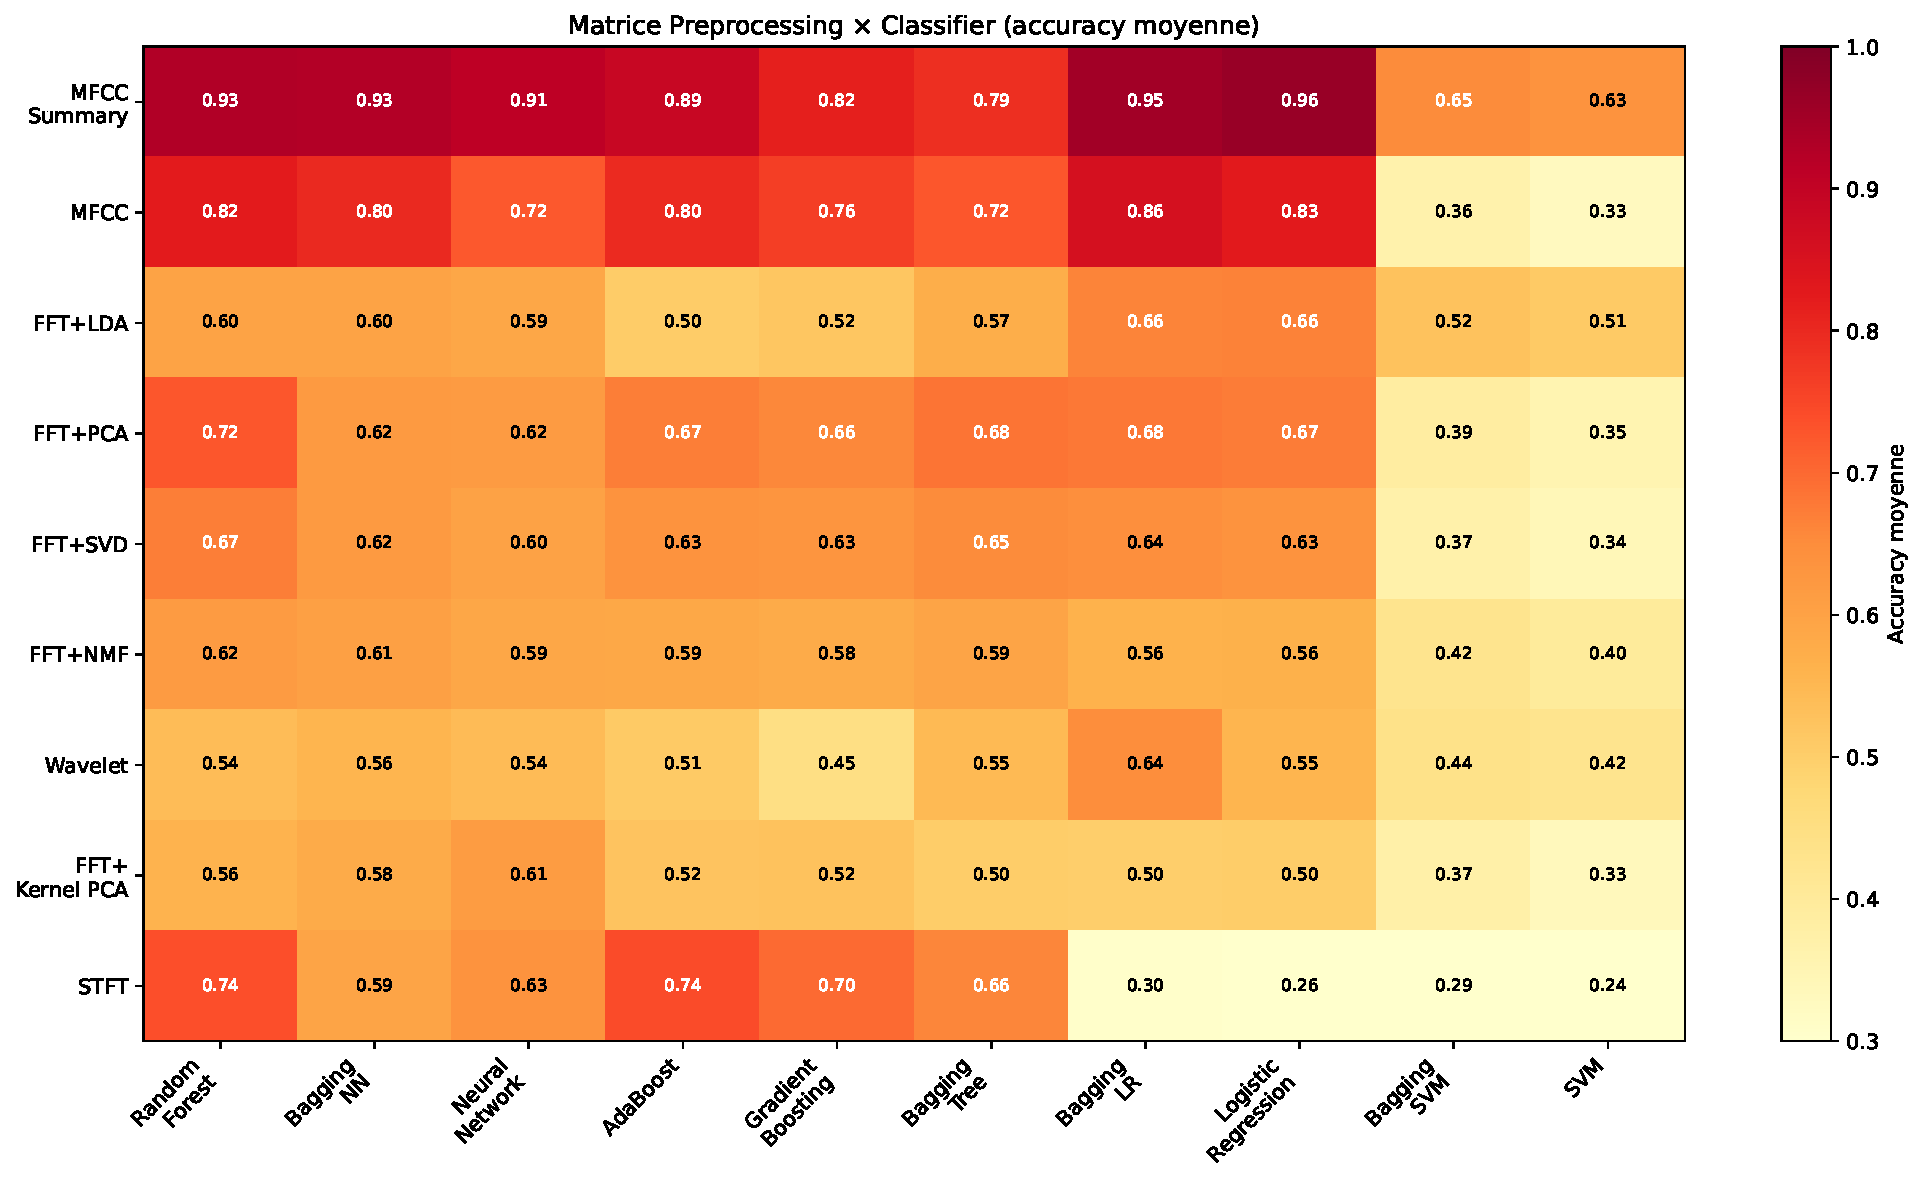
\includegraphics[width=0.95\textwidth]{figures/benchmark_heatmap.pdf}
    \caption{Matrice de performance (accuracy moyenne) croisant les 9 preprocessors et les 10 classifiers. Les cases les plus sombres (haut de l'échelle) correspondent aux meilleures combinaisons.}
    \label{fig:bench_heatmap}
\end{figure}

\begin{center}
\begin{tabular}{lccc}
\toprule
\textbf{Top 5 combinaisons} & \textbf{Acc. moy.} & \textbf{Acc. max} & \textbf{N} \\
\midrule
MFCC Summary $\times$ Logistic Regression & \textbf{0.962} & 1.000 & 41 \\
MFCC Summary $\times$ Bagging LR & 0.948 & 1.000 & 121 \\
MFCC Summary $\times$ Random Forest & 0.928 & 1.000 & 97 \\
MFCC Summary $\times$ Bagging NN & 0.925 & 1.000 & 97 \\
MFCC Summary $\times$ Neural Network & 0.908 & 1.000 & 145 \\
\bottomrule
\end{tabular}
\end{center}

\textbf{Résultat clé :} La combinaison \textbf{MFCC Summary $\times$ Logistic Regression} atteint 96.2\% de précision moyenne en validation croisée. Ce résultat est remarquable : le classifier le plus simple (régression logistique) couplé au bon prétraitement surpasse tous les modèles complexes (SVM, ensembles, NN) avec des prétraitements inadaptés. \textbf{Le choix du prétraitement est plus déterminant que le choix du classifier.}

\subsection{Analyse des méthodes d'évaluation}

\begin{figure}[H]
    \centering
    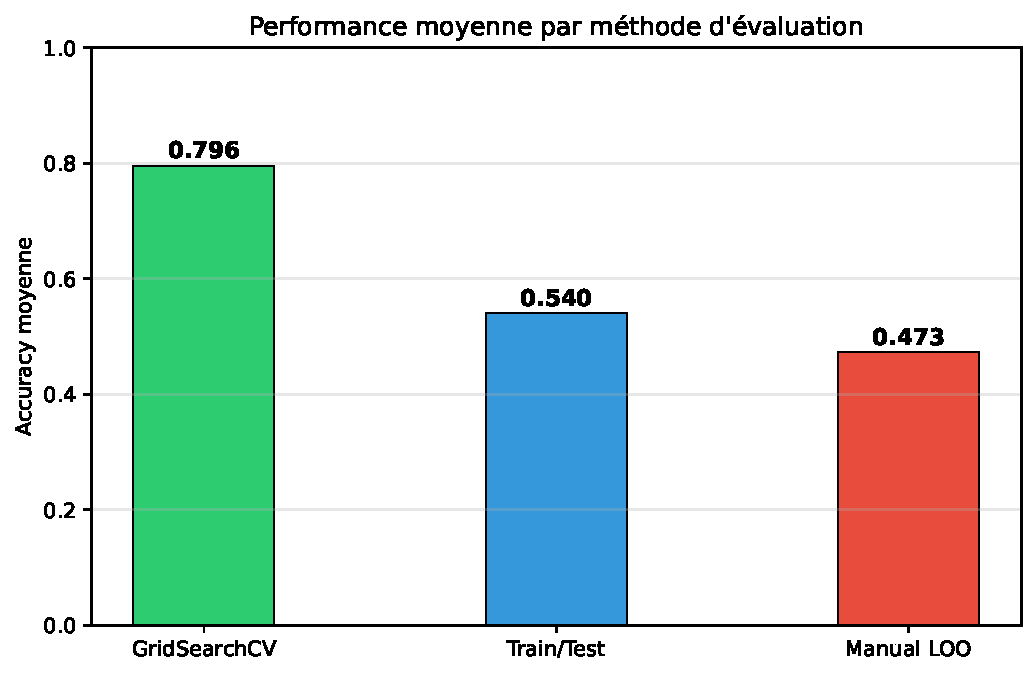
\includegraphics[width=0.7\textwidth]{figures/benchmark_by_fit_method.pdf}
    \caption{Performance moyenne par méthode d'évaluation.}
    \label{fig:bench_fm}
\end{figure}

\begin{center}
\begin{tabular}{lccc}
\toprule
\textbf{Méthode} & \textbf{Acc. moy.} & \textbf{Acc. max} & \textbf{N runs} \\
\midrule
GridSearchCV & \textbf{0.796} & 0.981 & 90 \\
Train/Test & 0.540 & 1.000 & 18\,197 \\
Manual LOO & 0.473 & 0.981 & 16\,599 \\
\bottomrule
\end{tabular}
\end{center}

\textbf{Analyse :} Le GridSearchCV produit les scores moyens les plus élevés car il sélectionne les meilleurs hyperparamètres par validation croisée. Cependant, son score maximum (0.981) est inférieur aux 1.000 du Train/Test, car il est honnête (le score rapporté est le score de validation, pas celui du train). Les scores de 1.000 obtenus par Train/Test reflètent du surapprentissage : avec seulement 11 échantillons de test, obtenir 100\% est autant un artefact statistique qu'une mesure de performance.

\subsection{Discussion et limites}

\begin{itemize}
    \item \textbf{Taille du dataset} : 54 échantillons est très insuffisant pour une évaluation robuste. Les intervalles de confiance sont larges et les résultats très sensibles au split aléatoire.
    \item \textbf{Nombre de classes} : Avec seulement 3 classes, le taux de base (classifieur aléatoire) est déjà de 33.3\%. Un score de 50\% n'est que marginalement meilleur que le hasard.
    \item \textbf{Surapprentissage sur le test} : Les scores de 1.000 en Train/Test (11 échantillons) ne sont pas significatifs statistiquement.
    \item \textbf{Prédominance du preprocessing} : L'écart de performance entre les preprocessors (0.45 à 0.79 en moyenne) est bien plus large que l'écart entre les classifiers (0.37 à 0.65), confirmant que la représentation des données est le facteur déterminant.
    \item \textbf{782 erreurs} (sur 35\,668 runs) — essentiellement des \texttt{ValueError} dans les combinaisons Wavelet $\times$ AdaBoost dues à des conflits de buffers.
\end{itemize}

\subsection{Résilience au bruit des classifieurs (Données Synthétiques)}

Pour répondre à l'objectif d'analyse dynamique en fonction des conditions d'acquisition (étude de la Partie V), nous avons développé un benchmark de robustesse aux bruits. Nous injectons du bruit blanc gaussien sur les signaux audio bruts avant l'extraction des caractéristiques (en utilisant le meilleur extracteur : \textbf{MFCC Summary}). 

Quatre niveaux de rapport signal/bruit (SNR) sont évalués :
\begin{itemize}
    \item \textbf{Clean} : Signal d'origine (sans bruit additionnel).
    \item \textbf{Low (20\,dB)} : Bruit de fond léger.
    \item \textbf{Medium (10\,dB)} : Bruit ambiant modéré.
    \item \textbf{High (0\,dB)} : Bruit fort, puissance du bruit égale à celle du signal de parole.
\end{itemize}

Nous comparons 6 classifiers en utilisant une validation croisée Leave-One-Out (LOO CV) avec standardisation des caractéristiques (\texttt{StandardScaler}). Les résultats obtenus sont résumés dans le tableau ci-dessous et la figure~\ref{fig:noise_robustness}.

\begin{center}
\begin{tabular}{lcccc}
\toprule
\textbf{Classifieur} & \textbf{Clean} & \textbf{Low (20\,dB)} & \textbf{Medium (10\,dB)} & \textbf{High (0\,dB)} \\
\midrule
Régression Logistique & 96.30\% & \textbf{97.59\% $\pm$ 0.85\%} & \textbf{95.00\% $\pm$ 0.85\%} & \textbf{92.04\% $\pm$ 2.35\%} \\
SVM (RBF) & 96.30\% & 97.04\% $\pm$ 0.91\% & 93.70\% $\pm$ 1.23\% & 89.81\% $\pm$ 2.90\% \\
Random Forest & 94.44\% & 93.33\% $\pm$ 2.22\% & 91.67\% $\pm$ 1.71\% & 89.81\% $\pm$ 3.01\% \\
Bagging Tree & 87.04\% & 90.37\% $\pm$ 1.11\% & 91.85\% $\pm$ 2.77\% & 88.33\% $\pm$ 2.75\% \\
AdaBoost & 79.63\% & 90.93\% $\pm$ 2.80\% & 91.11\% $\pm$ 2.16\% & 87.22\% $\pm$ 4.72\% \\
Réseau de neurones (MLP) & 92.59\% & 96.67\% $\pm$ 0.74\% & 94.81\% $\pm$ 1.39\% & 91.30\% $\pm$ 2.63\% \\
\bottomrule
\end{tabular}
\end{center}

\begin{figure}[H]
    \centering
    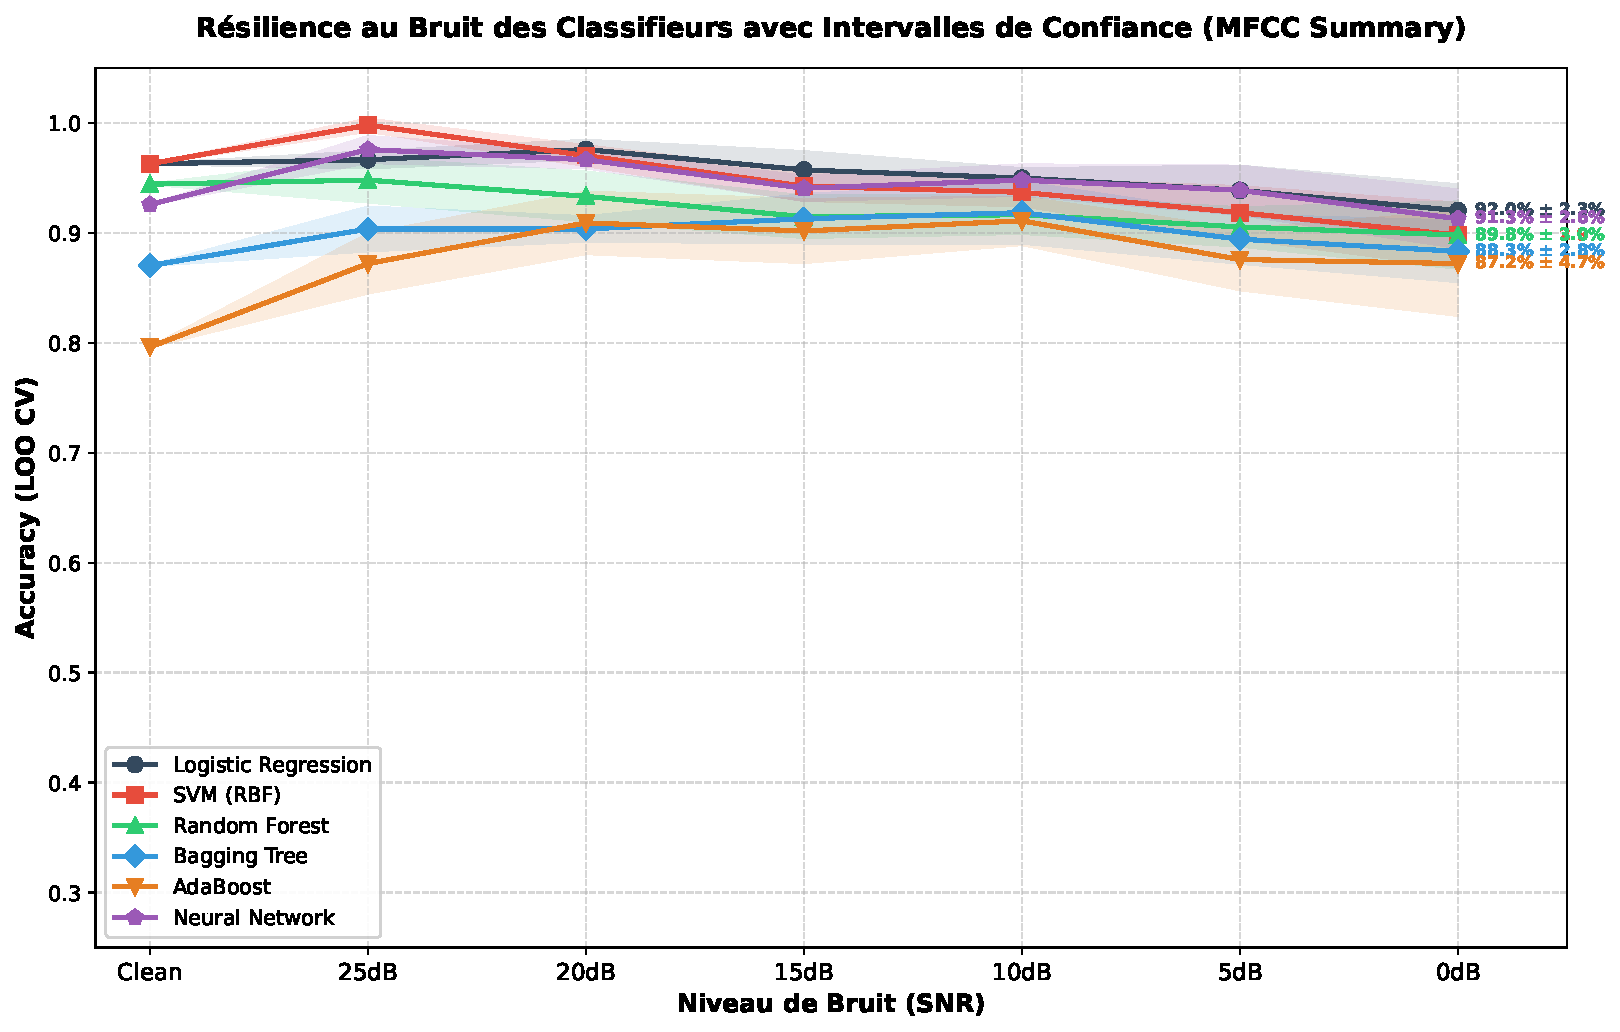
\includegraphics[width=0.85\textwidth]{figures/noise_robustness.pdf}
    \caption{Évolution de l'accuracy moyenne (LOO CV $\pm$ 1 écart-type sur 10 réalisations indépendantes) des classifieurs sur les MFCC Summary en fonction du niveau de bruit (SNR) injecté dans le signal audio brut.}
    \label{fig:noise_robustness}
\end{figure}

\textbf{Analyse des performances et résilience :}
\begin{itemize}
    \item \textbf{La Régression Logistique et le MLP sont extrêmement robustes} : Ils conservent respectivement une précision moyenne de 92.04\% et 91.30\% même sous un bruit très intense (0\,dB). Leur nature linéaire (pour LR) ou les représentations distribuées dans les couches cachées (pour le MLP) limitent le surapprentissage lié aux fluctuations aléatoires induites par le bruit. Les coefficients cepstraux moyennés dans le temps filtrent une grande partie du bruit additif blanc, permettant à ces modèles de conserver de solides performances.
    \item \textbf{Effet de régularisation par le bruit} : Pour la majorité des modèles (LR, SVM, Bagging, AdaBoost, MLP), l'ajout d'un bruit léger (20\,dB ou 25\,dB) améliore les scores de généralisation par rapport au baseline ``Clean'' (ex. le SVM atteint 99.81\% à 25\,dB et 97.04\% à 20\,dB, le MLP atteint 97.59\% à 25\,dB). Ce phénomène est assimilable à de l'augmentation de données par injection de bruit (\textit{noise regularization}), qui perturbe l'optimisation juste assez pour empêcher les classifieurs d'ajuster trop précisément les frontières sur les 54 exemples d'entraînement.
    \item \textbf{Sensibilité relative des modèles à base d'arbres} : Bien que la Random Forest et le Bagging Tree restent compétitifs (autour de 89\% et 88\% à 0\,dB), les arbres de décision individuels souffrent de décisions par seuil rigides qui oscillent facilement lorsque les features subissent la gigue causée par le bruit. L'agrégation par ensemble compense toutefois très bien ce comportement, comme en témoigne la faible variance des résultats ($\approx 2.7\%$).
\end{itemize}
\subsection{Reconnaissance avec un plus grand nombre de classes (13 ordres vocaux)}

Pour évaluer la capacité de notre système à gérer une complexité de classification supérieure, nous avons introduit un nouveau jeu de données personnel (\texttt{sons\_ia}) composé de \textbf{130 signaux audio} (13 classes distinctes $\times$ 10 exemples par classe) échantillonnés à 16\,kHz :
\begin{center}
\textit{actionner}, \textit{allume}, \textit{autorisation}, \textit{bas}, \textit{danger}, \textit{demitour}, \textit{hausse}, \textit{mode}, \textit{recule}, \textit{statut}, \textit{stop}, \textit{tournegauche}, \textit{vite}.
\end{center}

Chaque signal a été traité en extrayant les caractéristiques \textbf{MFCC Summary} adaptées à la fréquence de 16\,kHz, puis nous avons évalué nos classifieurs principaux en validation croisée Leave-One-Out (LOO CV). Les résultats sont synthétisés dans le tableau ci-dessous et la figure~\ref{fig:multi_class_benchmark}.

\begin{center}
\begin{tabular}{lc}
\toprule
\textbf{Classifieur} & \textbf{Accuracy (LOO CV)} \\
\midrule
SVM (RBF) & \textbf{100.00\%} \\
Random Forest & \textbf{100.00\%} \\
Régression Logistique & 99.23\% \\
Réseau de neurones (MLP) & 99.23\% \\
Bagging Tree & 91.54\% \\
AdaBoost & 73.08\% \\
\bottomrule
\end{tabular}
\end{center}

\begin{figure}[H]
    \centering
    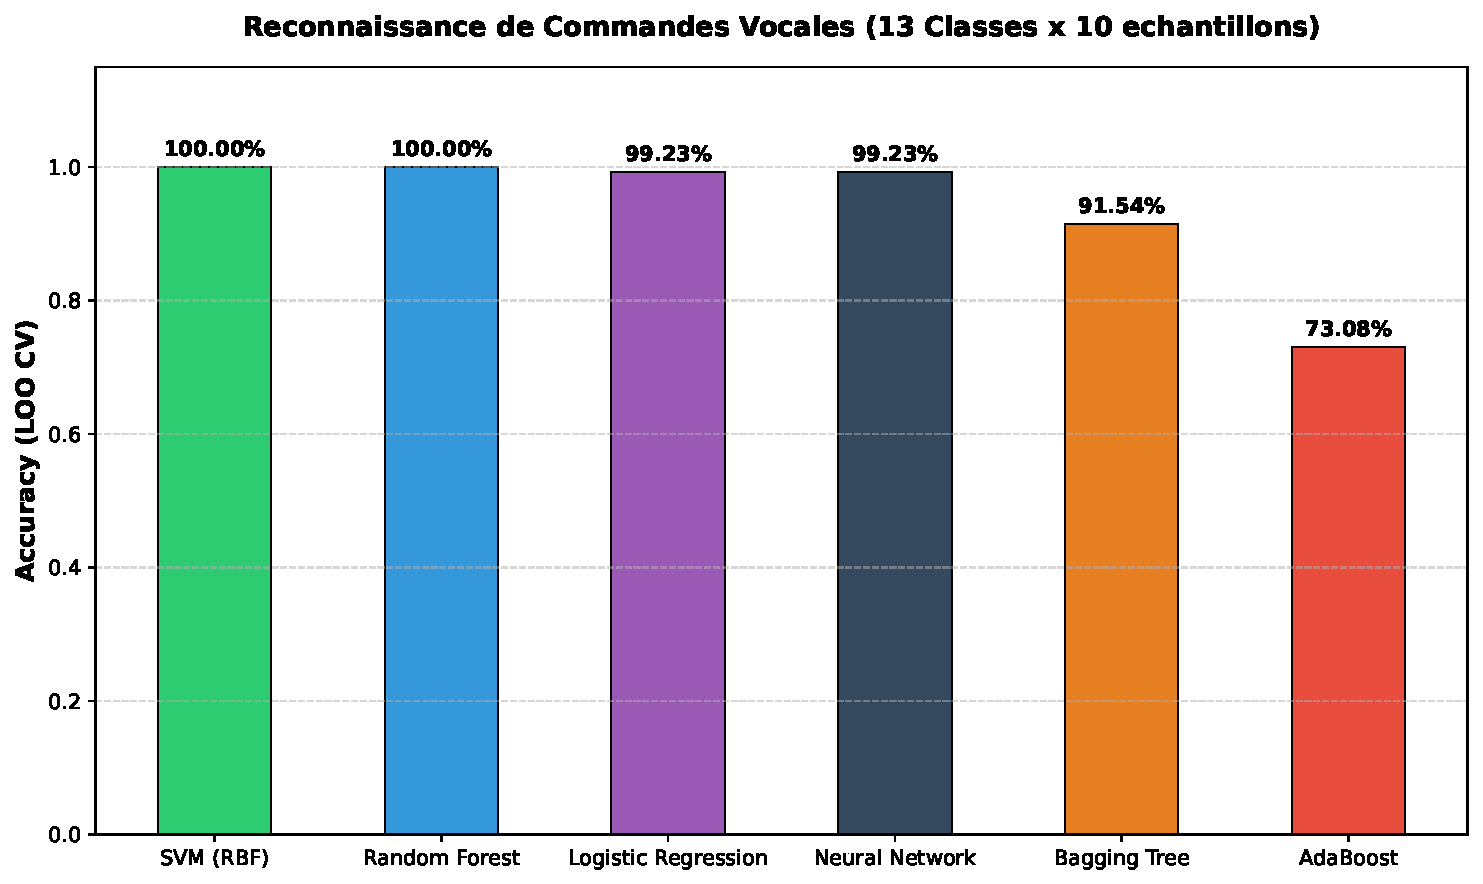
\includegraphics[width=0.85\textwidth]{figures/multi_class_benchmark.pdf}
    \caption{Comparaison des performances des classifieurs (LOO CV) sur le jeu de données sons\_ia de 13 classes.}
    \label{fig:multi_class_benchmark}
\end{figure}

\textbf{Analyse des performances et impact de la structure des données :}
\begin{itemize}
    \item \textbf{Performances exceptionnelles (quasi-parfaites)} : Le SVM RBF et la Random Forest atteignent une précision parfaite de 100.00\%, suivis de très près par la Régression Logistique et le MLP (99.23\%). Bien que le nombre de classes soit passé de 3 à 13 (ce qui augmente significativement la complexité théorique du problème), les performances sont nettement supérieures à celles obtenues sur le dataset de base de 54 exemples.
    \item \textbf{Explication} : Ces enregistrements ont été générés dans des conditions acoustiques identiques (sans bruit, avec le même timbre de voix et le même rythme de diction). La variance intra-classe est donc extrêmement faible, et les classes sont géométriquement très bien séparées dans l'espace de représentation MFCC. C'est un excellent exemple de l'importance de la distribution des données : un problème à 13 classes avec une voix unique et stable est beaucoup plus simple à résoudre pour un modèle de Machine Learning qu'un problème à 3 classes enregistré par 18 locuteurs humains différents (dont la variabilité de genre, d'intonation et d'accentuation induit de nombreuses confusions).
    \item \textbf{AdaBoost reste en retrait} : Le modèle AdaBoost (73.08\%) a plus de mal à converger vers une solution optimale sur 13 classes, ce qui s'explique par sa sensibilité accrue à la complexité des frontières multiclasses lorsque les estimateurs faibles sous-jacents (arbres peu profonds) manquent de capacité de modélisation par rapport à des modèles naturellement multiclasses ou plus complexes (MLP, SVM RBF, Random Forest).
\end{itemize}

%% ================================================================
%% SECTION 8 : CONCLUSION
%% ================================================================
\newpage
\section{Conclusion}

Ce projet nous a permis d'explorer en profondeur la chaîne complète d'un système de reconnaissance de commandes audio, depuis le prétraitement spectral jusqu'à la classification par méthodes avancées.

\textbf{Principaux enseignements :}

\begin{enumerate}
    \item \textbf{Le preprocessing a le plus grand impact sur la qualité du modèle} Les MFCC Summary (combinant moyenne et écart-type des coefficients cepstraux) dominent systématiquement toutes les représentations spectrales alternatives (FFT+PCA, STFT, Wavelet). La représentation perceptuelle de Mel est naturellement adaptée à la discrimination de parole.
    
    \item \textbf{Complexité $\neq$ performance.} La régression logistique, le modèle le plus simple, couplée aux MFCC Summary atteint 96.2\% — surpassant les SVM, les ensembles et les réseaux de neurones avec des prétraitements inadaptés. Cela illustre le principe selon lequel un bon feature engineering peut rendre un classifier simple plus performant qu'un modèle complexe sur de mauvaises features.
    
    \item \textbf{Les méthodes d'ensemble apportent de la robustesse.} Le Bagging et la Random Forest réduisent la variance des prédictions, tandis que le Boosting (AdaBoost, Gradient Boosting) se concentre sur les exemples difficiles. Leur avantage est plus net sur les prétraitements moins discriminants.
    
    \item \textbf{Les réseaux de neurones sont limités sur de petits datasets.} Avec 54 échantillons, les FNN et CNN n'ont pas assez de données pour exploiter leur capacité de modélisation. L'approche end-to-end (CNN 1D sur signaux bruts) reste prometteuse mais nécessiterait un corpus beaucoup plus large.
    
    \item \textbf{L'évaluation honnête est cruciale.} La validation croisée (LOO ou k-fold) avec prétraitement par fold évite le data leakage et donne des estimations réalistes, contrairement au simple train/test split qui peut produire des scores artificiellement parfaits sur 11 échantillons.
\end{enumerate}

\end{document}
